%\documentclass{sig-alternate-10pt}
\documentclass[10pt]{sig-alternate-05-2015}
\usepackage{balance}
\usepackage[breaklinks=true,colorlinks=true,plainpages=false,citecolor=blue,urlcolor=blue,filecolor=blue]{hyperref}
\usepackage{url}        % Not compatible with hyperref?
\usepackage{float}
\usepackage{graphicx}
\usepackage{amsmath}
\usepackage{color}
\usepackage{times}
\usepackage[sort]{natbib}
\usepackage{enumitem}
%\usepackage{subfigure}
\usepackage{verbatim}
\usepackage{xspace}
\usepackage{xfrac}
\usepackage{algorithmic} % must come after hyperref
\usepackage{algorithm}

\usepackage{listings}
%\usepackage{microtype} %does typographical voodoo to get rid of most overfull
                       %boxes. Ideally requires pdfTeX 1.4+, going directly
                       %to pdf. Don't use a DVI workflow.
\usepackage{balance}   %\balance keywork has to be included in the last page that
                       % will not be balanced, in the first column.
\usepackage{datetime}
\usepackage{morefloats}

\usepackage{caption}
\usepackage{subcaption}

\DeclareMathVersion{mathchartertext}
\SetSymbolFont{letters}{normal}{OML}{mdbch}{m}{n}
\newcommand{\gchar}[1]{\mathversion{mathchartertext}$#1$\mathversion{normal}}

% Configure algorithmic and listings
\renewcommand{\algorithmicrequire}{\textit{Input:}}
\renewcommand{\algorithmicensure}{\textit{Output:}}
\lstset{%language=Python,
numberstyle=\footnotesize,
basicstyle=\ttfamily\scriptsize,
numbers=left,
stepnumber=1,
showstringspaces=false,
breaklines=true}

 \newcommand{\todo}[1]{\textcolor{blue}{\textbf{TODO:} #1}}
 \newcommand{\eric}[1]{\textcolor{red}{\textbf{Eric:} #1}}
 \newcommand{\aditya}[1]{\textcolor{red}{\textbf{Aditya:} #1}}
 \newcommand{\keqiang}[1]{\textcolor{red}{\textbf{Keqiang:} #1}}
\newcommand{\cut}[1]{}

%\newcommand{\todo}[1]{}
\newcommand{\jeff}[1]{}
\newcommand{\colin}[1]{}
\newcommand{\brent}[1]{}

\newcommand{\eg}{\emph{e.g.}\xspace}
\newcommand{\cf}{{cf.}\xspace}
\newcommand{\ie}{\emph{i.e.}\xspace}
\newcommand{\etal}{{et al.}\xspace}

\hyphenation{light-weight}
\hyphenation{meas-ure-ment}
\newcommand{\tightparagraph}[1]{\vspace{5pt}\noindent\textbf{#1}\ }

%ejr, adding per jitu's email
\setlength{\pdfpagewidth}{8.5in}
\setlength{\pdfpageheight}{11in}


%don't want date printed
\date{}


%\title{Presto: Distributed Flowcell Load Balancing at the \\ Datacenter Network Edge}

\title{Presto: Edge-based Load Balancing for Fast Datacenter Networks}
%\author{Paper \#349, 12 pages + 1 page references}

\author{
{Keqiang He$^\dagger$ \hspace{0.2in} Eric Rozner$^\ast$ \hspace {0.2in} Kanak Agarwal$^\ast$}\\[.2cm]
{Wes Felter$^\ast$ \hspace{0.1in} John Carter$^\ast$ \hspace{0.1in} Aditya Akella$^\dagger$}\\\\
{\affaddr{$^\dagger$University of Wisconsin--Madison \hspace{0.15in} $^\ast$IBM Research}}
}

\newfont{\mycrnotice}{ptmr8t at 7pt}
\newfont{\myconfname}{ptmri8t at 7pt}
\let\crnotice\mycrnotice%
\let\confname\myconfname%


\clubpenalty=10000
\widowpenalty = 10000

\begin{document}

%%%%%%%%%%%%copy the following block from sigcomm15 instruction email's sample file, hek%%%%%
% Copyright
%\setcopyright{acmcopyright}
%\setcopyright{acmlicensed}
%\setcopyright{rightsretained}
%\setcopyright{usgov}
%\setcopyright{usgovmixed}
%\setcopyright{cagov}
%\setcopyright{cagovmixed}


% DOI
%\doi{10.475/123_4}

% ISBN
%\isbn{123-4567-24-567/08/06}

%Conference
%\conferenceinfo{SIGCOMM'15}{August 17--21, 2015, London, UK}

%\acmPrice{\$15.00}

\setcopyright{acmlicensed}
\conferenceinfo{SIGCOMM'15,}{August 17--21, 2015, London, United Kingdom}
\isbn{978-1-4503-3542-3/15/08}\acmPrice{\$15.00}
\doi{http://dx.doi.org/10.1145/2785956.2787507}
%
% --- Author Metadata here ---
%\conferenceinfo{SIGCOMM}{'15 London, UK}
%\CopyrightYear{2007} % Allows default copyright year (20XX) to be over-ridden - IF NEED BE.
%\crdata{0-12345-67-8/90/01}  % Allows default copyright data (0-89791-88-6/97/05) to be over-ridden - IF NEED BE.
% --- End of Author Metadata ---

%%%%%%%%%%%end of sample file block from sigcomm'15 instrction email%%%%%%
\maketitle

\begin{abstract}

Multi-tenant datacenters are successful because tenants 
can seamlessly port their applications and services
to the cloud. Virtual Machine (VM) technology plays an integral role in this success
by enabling a diverse set of software to be run on a unified underlying framework. This
flexibility, however, comes at the cost of dealing with out-dated, inefficient, or 
misconfigured TCP stacks implemented in the VMs. This paper investigates if
administrators can take control of a VM's TCP congestion control
algorithm {\em without} making changes to the VM or network hardware.
We propose~\acdc{} TCP, a scheme that exerts fine-grained
control over arbitrary tenant TCP stacks by enforcing per-flow congestion
control in the virtual switch (vSwitch). Our scheme is light-weight, flexible, scalable and
can police non-conforming flows. In our evaluation the computational overhead
of~\acdc{} TCP is less than~\crs{one percentage point} and we show implementing an administrator-defined congestion control algorithm
in the vSwitch (\ie{}DCTCP) closely tracks its native performance, regardless of the VM's TCP stack. 


\end{abstract}

%%%%%%%%%copied from sigcomm'15 sample file, CCS, new for sigcomm15, hek%%%%%%

%
% The code below should be generated by the tool at
% http://dl.acm.org/ccs.cfm
% Please copy and paste the code instead of the example below. 
%

\begin{CCSXML}

<ccs2012>

<concept>

<concept_id>10003033.10003034</concept_id>

<concept_desc>Networks~Network architectures</concept_desc>

<concept_significance>500</concept_significance>

</concept>

<concept>

<concept_id>10003033.10003058.10003064</concept_id>

<concept_desc>Networks~End nodes</concept_desc>

<concept_significance>500</concept_significance>

</concept>

<concept>

<concept_id>10003033.10003099.10003102</concept_id>

<concept_desc>Networks~Programmable networks</concept_desc>

<concept_significance>500</concept_significance>

</concept>

<concept>

<concept_id>10003033.10003106.10003110</concept_id>

<concept_desc>Networks~Data center networks</concept_desc>

<concept_significance>500</concept_significance>

</concept>

<concept>

<concept_id>10003033.10003068.10003069</concept_id>

<concept_desc>Networks~Data path algorithms</concept_desc>

<concept_significance>300</concept_significance>

</concept>

<concept>

<concept_id>10003033.10003079.10003082</concept_id>

<concept_desc>Networks~Network experimentation</concept_desc>

<concept_significance>300</concept_significance>

</concept>

</ccs2012>

\end{CCSXML}



\ccsdesc[500]{Networks~Network architectures}

\ccsdesc[500]{Networks~End nodes}

\ccsdesc[500]{Networks~Programmable networks}

\ccsdesc[500]{Networks~Data center networks}

\ccsdesc[300]{Networks~Data path algorithms}

\ccsdesc[300]{Networks~Network experimentation}

%
% End generated code
%

%
%  Use this command to print the description
%
\printccsdesc

% We no longer use \terms command
%\terms{Theory}

\keywords{Load Balancing; Software-Defined Networking; %TCP Segment Offload; Generic Receive Offload}
}
%%%%%%%%%%%%%%%%%%%%%%%%%%%%%%%%%%%%%%%%%%%%%%%%%%%%%%%%%%%%%%%%%%%%%%%%%%%%%%
\chapter{Introduction}
\label{chap:intro}
Over the past few years, cloud-based networking solutions have been gaining widespread acceptance and
deployment for organizations such as enterprises and institutions~\cite{paxson1997end}.

\section{Cloud Infrastructure Organization}
% virtual network data plane

%While our work applies to general cloud networking settings, for the purposes of 
In this thesis, we focus on multi-tenant cloud data centers.
In this setting, tenants deploy \emph{virtual private clusters}
composed of application end-points (this could be service software in

\section{Challenges in Diagnosing Cloud Networks}
\label{sec:intro:challenges}
Troubleshooting network problems is difficult. A network is a distributed

\begin{itemize}
\item Cloud networks have higher complexity than traditional networks.  In data planes, network virtualization introduces more software components, including software switches, hypervisors, and so on; software middleboxes are introduced to support network function virtualization. In control planes, the cloud controllers need to perform more functions to set up virtual networks; the controllers map tenants' requirements from a logical view to a physical view, and finally to devices rules. Cloud networks involve a greater number of components involved, and these components may have logical or physical dependency (e.g., exchanging data or sharing hardware resources). This complexity in cloud networks makes them not only more error-prone but also difficulty to manage and diagnose.
\item The two roles in cloud networks makes the management trickier than traditional network. The two roles are the provider (or operator) and the tenants, and their information is isolated from each
other. In the case of network problems, the interaction between the provider and
the tenants is crucial for problem solving; however, this process is usually of low efficiency. 
The tenants observe misbehaviors of their applications directly, but they lack diagnostic tools.
The provider does not know the applications' performance, so they can only wait for tenants' tickets.
%Due to the isolation, both parties cannot perform a complete diagnosis; therefore, 
The two parties need to exchange observations to figure out the problem. This manual process increases
the problem-solving time and maintenance cost.
\item The visibility of cloud networks is not well provided to customers and operators. In traditional networks, network devices and components provide various information for operators to monitor or troubleshoot, e.g., packet drop statistics in switches and the network protocol stack. However, by our study, this kind of visibility is not well preserved in cloud networks. For customers, the cloud provider does not provide visibility of how their packets traverse the network for security reasons. For the provider, some virtualization components are introduced to cloud networks without keeping the visibility for diagnosis\textemdash there are several silent packet drops in VM hypervisors and software middleboxes. This is partially due to the fact that developers typically focus on functionality instead of diagnostic features in the first few versions of the software.
\end{itemize}


\section{An Overview of Our Approach}
\label{sec:intro:approach}
Ever since the birth of networks, network problems have been appearing and upseting network operators. There have been numerous proposals aiming to solve various problems. For example, there are standards or technologies such as SNMP, sFlow, and NetFlow to collect states in networks; there are network models and diagnostic algorithms to discover culprits in network problems; and there are various network diagnostic solutions for traditional networks and software-defined networks, which combine the technologies and algorithms. These approaches are undoubtedly valuable in their specific scenarios.

However, these solutions do not overcome the challenges in diagnosing cloud networks (Section~\ref{sec:intro:challenges}). In this thesis, we make a study of problems in cloud networks. According to the cloud organization, we look into each planes and summarize new problems. In more details, we found that in application planes, the isolation between tenants and the provider causes tenants unable to diagnose their virtual networks, thus we propose, design and implement a virtual network diagnostic service in application planes. We found that in data planes, increasing complexity and lack of visibility cause performance problems difficult to be identified, thus we modify software data planes, collect statistics and leverage the statistics to perform accurate diagnosis. We also find inconsistency issues in control planes, where tenant requirements may not be consistency with physical device states; we leave this problem in future works.

Decomposing cloud networks into three planes and reconsidering diagnostic challenges in cloud networks is an efficient way to discover, abstract and solve cloud network problems. We feel that, owing to our approach, several cloud-specific problems are discovered. Therefore, our works improve the reliability of cloud networks.

\section{Thesis Outline}
\label{sec:intro:outline}
The rest of this thesis is organized as follows. 
In Chapter~\ref{chap:background}, we make a study of cloud network problems and briefly describe our approaches.
In Chapter~\ref{chap:vnd},
we describe our design of the virtual network diagnostic service. In Chapter~\ref{chap:perfsight},
we present our solution for software data plane diagnosis.
In Chapter~\ref{chap:related}, we discuss the related work, 
Finally in Chapter~\ref{chap:conc}, we conclude this thesis and discuss options for future work.

\section{Design Decisions and Challenges}
\label{sec:background}

In Presto, we make several design choices to 
build a highly robust and scalable system that provides near optimal load 
balancing without requiring changes to the transport layer or switch hardware. We 
now discuss our design decisions.


\subsection{Design Decisions}

\tightparagraph{Load Balancing in the Soft Edge} A key design decision in Presto 
is to implement the functionality in the soft edge (\ie{}the vSwitch and hypervisor) of 
the network. 
%should we motivate why not to do it in hardware?
%A current trend in datacenter design is to utilize network equipment from 
%original design manufacturers (ODMs) in order to simplify and customize
%the network. This has been reported to significantly reduce costs and improve
%network performance~\cite{aws-peek}.
%Motivation here is that network is becoming very simple, and functionalities
%are being moved to an intelligent edge. Examples are VMWare/NSDI, Fabric, NFV in vSwitch,
%SDNs/OpenFlow, 
% Given recent advancements in this space\eric{what advancements? can we be more specific
% in order to provide better motivation?}, we believe the soft edge is the best 
% place to deploy new network functions, such as load balancing, in a scalable and 
% distributed manner.\eric{is this a new position? vmware nsdi paper...}
The vSwitch occupies a unique position in the networking stack 
in that it can easily modify packets without requiring any changes to customer VMs or transport layers.
Functionality built into the vSwitch can be made aware of the underlying hardware offload
features presented by the NIC and OS, meaning it can be fast.
Furthermore, an open, software-based approach prevents extra hardware cost and vendor 
lock-in, and allows for simplified network management. 
These criteria are important for providers today~\cite{aws-peek}.
Thanks to projects like Open vSwitch, 
soft-switching platforms are now fast, mature, open source, adopted widely, remotely 
configurable, SDN-enabled, and feature-rich~\cite{ovs-edge,nv-mtd,pfaff2015design}. Presto is built on these 
platforms.

\tightparagraph{Reactive vs Proactive Load Balancing} The second major design decision in 
Presto is to use a proactive approach to congestion management. Bursty 
behavior can create transient congestion that must be reacted to 
before switch buffers overflow to prevent loss (timescales range from 100s of $\mu$s 
to around 4 ms~\cite{planck}). This requirement renders most of the centralized reactive schemes ineffective
as they are often too slow to react to any but the largest network events,~\eg{}link failures. 
%Not reacting to transient congestion can increase tail latencies.
Furthermore, centralized schemes can hurt performance when rerouting
flows using stale information.
%By reacting on a different scale than the congestion, centralized schemes may reroute flows
%on stale information, which can hurt performance.
Distributed reactive schemes like MPTCP~\cite{mptcp} and 
CONGA~\cite{conga} can respond to congestion at faster timescales, but have a high barrier to deployment.
Furthermore, distributed reactive schemes must take great care to avoid oscillations.
Presto takes a proactive, correct-by-design approach to congestion management. 
That is, if small, near-uniform portions of traffic are equally
balanced over a symmetric network topology, then the load-balancing can remain agnostic to congestion and
leave congestion control to the higher layers of the networking stack.
%then we don't need to 
%be reactive to congestion.
Presto is only reactive to network events such as link failures. Fortunately, 
the larger timescales of reactive feedback loops are sufficient in these scenarios. 

\tightparagraph{Load Balancing Granularity} ECMP has been shown to be ineffective at load balancing the network, and thus many schemes advocate load balancing at a finer granularity than a flow~\cite{drb,conga,juniper-vcf,packetspray}. A key factor impacting the choice of granularity is operating at high speed. 
%and ensuring suitable application level performance.
%Implementing fine-grained, near-uniform load balancing in 10+ Gbps networks
%is difficult.
Operating at 10+ Gbps incurs great computational overhead, and therefore host-based load balancing schemes
must be fast, light-weight and take advantage of optimizations provided in the networking stack.
For example, per-packet load balancing techniques~\cite{drb} cannot be
employed at the network edge because TSO does not work on a per-packet
basis. TSO, commonly supported in OSes and NICs, allows for large TCP segments (typically 64 KB in size)
to be passed down the networking stack to the NIC. The NIC breaks the segments into MTU-sized packets and copies and computes
header data, such as sequence numbers and checksums. When TSO is disabled, a host incurs 100\% utilization of one CPU core and can only achieve
around 5.5 Gbps~\cite{bullettrains}. Therefore, per-packet schemes are unlikely to scale to fast networks without hardware support.
Limiting overhead by increasing the MTU is difficult because
VMs, switches, and routers must all be configured appropriately, and traffic
leaving the datacenter must use normal 1500 byte packets. Furthermore, per-packet schemes~\cite{drb,packetspray} are likely to
introduce significant reordering into the network.
%Achieving line rate at 10 Gbps is nontrivial because dealing
%with so many 1500 byte MTU-sized packets at varying layers
%of the networking stack causes significant computational overhead.
%Therefore, modern operating systems and network adapters have many
%optimizations to help burden the load.
%On the sender side, TCP Segmentation Offload (TSO)~\footnote{Generically known as large segment offload or generic segmentation offload}
%is designed to allow the TCP/IP stack to deal with large TCP segments. Segments, up to 64 KB in size, are passed
%from the application layer all the way down to the NIC, which in turn breaks the large segment down into 1500 byte packets.
%The NIC copies and calculates the header information, such as checksums and sequence numbers.
%This allows the computational burden to be substainally lessened, and therefore rates of 10+
%Gbps can be achieved. With TSO disabled, achievable 10 Gbps throughput drops to around 5.5 Gbps~\cite{bullettrains}.



\begin{figure}[!t]
        \centering
  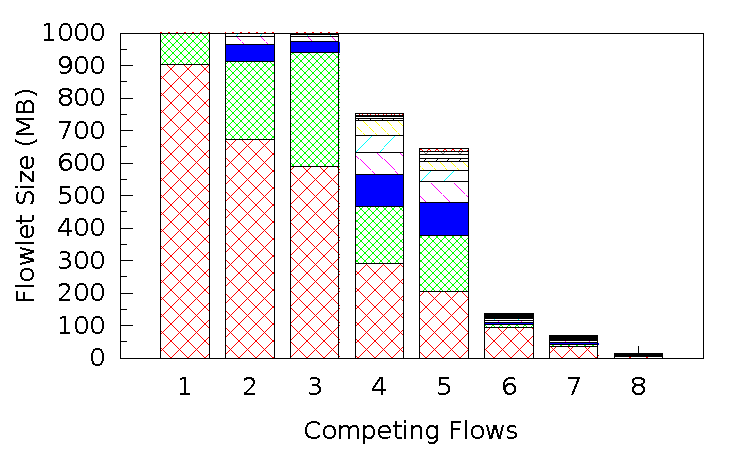
\includegraphics[width=0.7\textwidth]{presto/figures/flowlets/histo.pdf}
        \caption{Stacked histogram of flowlet sizes (in MB) for a 1 GB {\tt scp} file transfer. We vary the number of {\tt nuttcp}~\cite{nuttcp} background flows and
                denote them as {\em Competing Flows}. The size of each flowlet is shown within each bar, and flowlets
                are created whenever there is a 500 $\mu$s delay between segments. The top 10 flowlet sizes are shown here.
                We also analyzed the results of a 1 GB {\tt nuttcp}, {\tt ftp}, and a simple custom client/server transfer and found them
                to be similar. }
        \label{micro_flowlet_size}
\end{figure}

%\aditya{the following two paras don't flow well. they don't make a clear case for why flowlets is a bad idea and TSO segment level switching is a good idea. if reordering is the 100us flowlets' big problem then why not use our receiver-side reordering tricks with 100us flowlets? also it is not clear how were are overcoming reordering simply by relying on TSO segment switching}

%\eric{Rough estimates from our experiments with 100$\mu$s: ~90\% of flowlet sizes are 114KB or less with flowlets. ~00.1\% of flowlets are
%larger than 1 MB, with the largest ranging from 2.1-20.5MB. Some thoughts: (i) 100 $\mu$s flowlets can still have flowlet sizes larger 
%than switch buffers, which can cause congestion/loss when collision occur, (ii) given that flowlet with 100 $\mu$s does not prevent reordering,
%then why should we use flowlets at all? (iii) flowlets were really meant to have inactivity timers larger than the max difference in latency
%over any two paths, and buffer latency at one switch alone is ~4ms, so the use of flowlets on these small time scales is fundamentally
%flawed, (iv) flowlets are sensitive to traffic demand at sender, (v) flowlets are non-uniform in size, (vi) flowlets could break small 
%flows over multiple paths. Using TSO segment ensures: (i) small, uniform units of load-balancing, which means (ii) we are indenpendent
%of traffic demand, (iii) collisions are not a problem b/c TSO size is smaller than buffer size, (iv) most small flows are routed
%over the same path, (v) we do not impose too much computational overhead on sender/receiver and (vi) we still need to solve reordering.}

% Rough outline for next two paragraphs
% Problem with flowlets:
%  1. Sensitive to traffic patterns at the sender
%     a. In practice, we find this means the distribution of flowlet sizes is not uniform, and has a tail
%     b. These tails can still experience hash collisions, albeit less often.
%		i. congestion: lower throughput and to longer mice tail latencies
%  2. Needlessly break down small flows into several flowlets
%     a. Especially early in connection: 100us, 50 KB mice flows broken into 4-5 flowlets
%  3. Designed to be robust to reordering, but difficult to tune
%


Another possibility is to load balance on flowlets~\cite{conga,juniper-vcf}.  
A flow is comprised of a series of bursts, and a flowlet is created when
the inter-arrival time between two packets in a flow exceeds a threshold inactivity timer.  
In practice, inactivity timer values are between 100-500 $\mu$s~\cite{conga}. 
These values intend to strike a good balance between load balancing on a sub-flow level 
and acting as a buffer to limit reordering between flowlets.
Flowlets are derived from traffic patterns at the sender, and in practice this
means the distribution of flowlet sizes is not uniform. To analyze flowlet sizes, a simple experiment is shown in Figure~\ref{micro_flowlet_size}. 
We connect a sender and a receiver to a single switch and start an {\tt scp} transfer designed to 
emulate an elephant flow. Meanwhile, other senders are hooked up to the same switch and
send to the same receiver. We vary the number of these competing flows and show a stacked histogram of 
the top 10 flowlet sizes for a 1 GB {\tt scp} transfer with a 500 $\mu$s inactivity timer. 
The graph shows flowlet sizes can be quite large, with more than half the transfer being attributed
to a single flowlet for up to 3 competing flows. Using a smaller inactivity timer, such 100$\mu$s, helps (90\% of flowlet sizes are 114KB or less), but
does not prevent a long tail: 0.1\% of flowlets are larger than 1 MB, with the largest ranging from 2.1-20.5 MB.
Collisions on large flowlet sizes can lead to congestion.
The second problem with flowlets is that small inactivity thresholds, such as 100 $\mu$s, can lead to significant reordering.
Not only does this impact TCP performance (profiled in Section~\ref{sec:micro}), but it also needlessly 
breaks small flows into several flowlets. With only one flow in the network, we found a 50 KB
mice flow was broken into 4-5 flowlets on average. Small flows typically do not need to be
load balanced on a sub-flow level and need not be exposed to reordering.


%Another possibility is to load balance on flowlets~\cite{conga,juniper-vcf}.  A flow is typically comprised of a series of bursts, and each burst is defined as a flowlet. By monitoring the inter-arrival time of packets in a flow, one can easily define an inactivity timer to seperate flowlets.  In practice, intactivity timer values are between 100-500 $\mu$s~\cite{conga}. These values are intended to strike a good balance between creating enough opportunities to load balance on a sub-flow level and also ensure the reordering is limited at the destination due to the time buffer naturally incurred between flowlets.  We find, however, that it is difficult to strike a balance between achieving fine-grained, near-optimal load balancing and robustness against reordering. We perform a simple experiment in Figure~\ref{micro_flowlet_size}.  We connect a sender and a receiver to a single switch and start a transfer over an application designed to emulate an elephant flow ({\tt scp}). Meanwhile, we also hook up other senders to the same switch and have them send to the same reciever. We vary the number of competing flows and show a stacked histogram of the top 10 flowlet sizes for a 1 GB scp transfer with a 500 $\mu$s inactivity timer. \eric{Competing flows use nuttcp.} The graph shows flowlet sizes can be large, which means hash collisions can still occur on large flowlets.  Using a smaller timeout, such as 100 $\mu$s, creates smaller flowlets, but as we show in Section XXX, suffers from severe reordering that greatly reduces throughput and hurts applications.  \eric{mention creates congestion, which leads to lower thorughput and increase mice FCT latency}

% What do we want in sub-flow load balancing?
%  A. Want to move toward idealized ECMP: uniform sub-flow load balancing without the tail
%  B. Units should be as small as possible for fine-grained load balancing, but
%       not so small to be inefficient (TSO) or break small flows into parts
%  C. Independent of traffic patterns on sender
%  As a result, we settle on...

The shortcomings of the previous approaches lead us to reconsider on what granularity
load balancing should occur. 
%We take motivation from a best-case ECMP scenario. 
Ideally, sub-flow load balancing should be done on near uniform sizes.
%independent of traffic patterns on the sender to avoid long tails. 
Also, the unit of load balancing should be small to
allow for fine-grained load balancing, but not so small as to break small flows into 
many pieces or as to be a significant computational burden. As a result, we
propose load balancing on 64 KB units of data we call {\em flowcells}. Flowcells
have a number of advantages. First, the maximum segment size supported by TSO
is 64 KB, so flowcells provide a natural interface to high speed optimizations provided
by the NIC and OS and can scale to fast networking speeds. Second, an overwhelming fraction of mice flows are less than 64 KB in size
 and thus do not have to worry about reordering~\cite{benson10,vl2,kandula2009nature}.
Last, since most bytes in datacenter networks originate from elephant flows~\cite{kandula2009nature,benson10,dctcp},
this ensures that a significant portion of datacenter traffic is routed on uniform
sizes. While promising, this approach must combat reordering to be effective. 
Essentially we make a trade-off: 
%we provide line rate load balancing in the most effective
%manner as to avoid congestion and then handle reordering head-on at the receiver.
the sender avoids congestion by providing fine-grained, near-uniform load balancing,
and the receiver handles reordering to maintain line-rate.


%We highlight the challenges of this approach
%in the next subsection and provide a design to mitigate reordering problems in Section~\ref{sec:design}.

%In order to obtain fine-grained, near-optimal load balancing, we should stripe on a granularity
%that is indendpent of traffic patterns, near-uniform in size, and as small as possible while still
%scaling to fast network speeds.
%Therefore, we argue the TSO segment~\keqiang{what about saying maximum TSO segment size (64KB), each TSO segment's size is bounded by maximum TSO size} 
%is the natural granularity in which to load balance. Doing so
%provides several benefits. First, TSO segments are small and near-uniform in size, so an
%effective load-balancing scheme should be able to closely track the optimal case of per-packet
%load balancing, but without the additional computational overhead.
%Second, the TSO engine in the NIC will ensure that all packets created from a TSO segment will contain the same
%header information. We show in Section XXX how this is important to deal with reordering because
%we can easily impart metadata on all packets within a segment that help us distinguish loss from 
%ordering~\keqiang{all the packets within the same flowcell contain the same flowcell id.  
%"all packets created from a TSO segment will contain the same
%header information" is fine but a flowcell can contrain several TSO segments depending on TSO segment size}.
%Last, small flows less than 64 KB in size will actually be routed over the
%same path in the network, meaning a very large fraction of mice flows will not be routed on a subflow
%level and thus do not have to worry about reordering~\cite{benson10,vl2,kandula2009nature}~\keqiang{Around 90\% of datacenter flows' sizes are smaller than 64KB~\cite{benson10}, 
%meaning the overwhelming majority is load balanced like ECMP and we only need to engineering the left 10\%}.
%\eric{need to mention that we can combine segments as long as not above 64 KB, so not really
%per TSO segment. helps in small flows.}
%While promising, this approach has a major challenge: reordering. We highlight these challenges
%in the next subsection and provide a design to mitigate the problems in Section~\ref{sec:design}.

\tightparagraph{Per-Hop vs End-to-End Multipathing}
The last design consideration is whether multipathing should be done on a local, per-hop level (\eg{}ECMP), or
on a global, end-to-end level. In Presto, we choose the latter: pre-configured end-to-end paths
are allocated in the network and path selection (and thus multipathing) is realized by having the network edge
place flowcells onto these paths. 
Presto can be used to load-balance in an ECMP style per-hop manner, but the choice of end-to-end 
multipathing provides additional benefits due to greater control of how flowcells are mapped to
paths. Per-hop multipathing can be inefficient
under asymmetric topologies~\cite{wcmp}, and load-balancing on a global end-to-end level can allow
for weighted scheduling at the vSwitch to rebalance traffic. This is especially important when failure occurs.
The second benefit is flowcells can be assigned over multiple paths very evenly
by iterating over paths in a round-robin, rather than randomized, fashion. 

%As we show
%in Section~\ref{sec:micro}, randomization in per-hop multipathing can lead to "unluckiness" where
%multiple flowcells get sent to the same link over a small timescale by multiple flows. This transient congestion
%can lead to increased buffer occupancy and higher delays in the network. These benefits can
%fundamentally be provided at the per-hop level (\cite{wcmp} handles asymmetry), but require changes to networking firmware. 
%These considerations motivate us to utilize end-to-end multipathing, but Presto can also
%use per-hop multipathing when conveinent.

\subsection{Reordering Challenges}
%The above design decisions in Presto cause following main challenges:
Due to the impact of fine-grained, flowcell-based load balancing, Presto must account for reordering. Here, we 
highlight reordering challenges. The next section shows how Presto deals with these concerns.

%\tightparagraph{Soft Edge Distributed Load Balancing}
%There are two main challenges in implementing load balancing at the soft edge. First, the implementation
%must scale to fast networking speeds because networking at 10+ Gbps can have significant overhead if not carefully
%considered. Therefore, in order to achieve line rate, great care must be taken to ensure that load balancing
%schemes are light-weight, simple and can take advantage of optimizations provided by the NIC and OS.  
%The second major problem is how to load balance in a distributed fashion at the vSwitches in such
%a way that the load balancing performs well globally.
%Nodes must ensure they are spreading
%their traffic equally throughout the network, but in a low-overhead fashion that does not require detailed
%topographical information about the network, real-time traffic matrices, or strict coordination
%with other senders.

%\eric{several things to add: in presto, we can just make dumb edge decisions and not have to worry
%about (i) the traffic patterns, that is who else is sending, (ii) topology asymmetry. Basically,
%we want to highight that the vSwitch shouldn't require a lot of detailed network-wide information,
%but should be able to somehow still load balance in a way that performs very well globally.}

\tightparagraph{Reordering's Impact on TCP} The impact of reordering on TCP is well-studied~\cite{leung2007overview,paxson1997end}. 
Duplicate acknowledgments caused by reordering
can cause TCP to move to a more conservative sender state and reduce the sender's congestion window.
Relying on parameter tuning, such as adjusting the DUP-ACK threshold, is not ideal because 
increasing the DUP-ACK threshold increases the time to recover from real loss. Other TCP settings
such as Forward Acknowledgement (FACK) assume un-acked bytes in the SACK are lost and degrade
performance under reordering. 
A scheme that introduces reordering should not rely on careful configuration of TCP parameters
because (i) it is hard to find a single set of parameters that work effectively over multiple 
scenarios and (ii) datacenter tenants should not be forced to constantly tune their networking stacks.
Finally, many reordering-robust variants of TCP have been proposed~\cite{rr-tcp,blanton2002making,tcp-pr}, but
as we will show, GRO becomes ineffective under reordering. Therefore, reordering should
be handled below the transport layer.

\tightparagraph{Computational Bottleneck of Reordering}
Akin to TSO, Generic Receive Offload (GRO) mitigates the computational burden of receiving
1500 byte packets at 10 Gbps. GRO is implemented in the kernel of the hypervisor,
and its handler is called directly by the NIC driver. It is responsible
for aggregating packets into larger segments that are pushed up to OVS and the TCP/IP stack. 
GRO is implemented in the Linux kernel and is used even without virtualization. Similar
functionality can be found in Windows (RSC~\cite{ms-rsc}) and hardware (LRO~\cite{grossman2005large}).

Because modern CPUs use aggressive prefetching, the cost of receiving
TCP data is now dominated by per-packet, rather than per-byte, operations.
As shown by Menon~\cite{optimize-tcp-receive},  the majority of this overhead comes from
buffer management and other routines not related to protocol processing, and therefore 
significant computational overhead can be avoided by aggregating "raw" packets from
the NIC into a single {\tt sk\_buff}.
%\footnote{Refer to~\cite{linuxgro,optimize-tcp-receive} for detailed study and explanation}
Essentially, spending a few cycles to aggregate packets within GRO creates less segments for
TCP and prevents having to use substantially more cycles at higher layers in the networking stack.
Refer to~\cite{linuxgro,optimize-tcp-receive} for detailed study and explanation.

To better understand the problems reordering causes, a brief description of  
the TCP receive chain in Linux follows. First, interrupt coalescing allows the NIC to create an interrupt for a batch of packets~\cite{mogul1997eliminating,understanding-linux-network},
which prompts the driver to poll the packets into an aggregation queue. Next, the driver
invokes the GRO handler, located in the kernel, which
{\em merges} the packets into larger segments. The merging continues,
possibly across many polling events, until a segment
reaches a threshold size, a certain age, or cannot be combined with the incoming packet. Then, the
combined, larger segment is {\em pushed up} to the rest of the TCP/IP networking stack. The GRO process is
done on a per-flow level. With GRO disabled, throughput drops to around
5.7-7.1 Gbps and CPU utilization spikes to 100\% (Section~\ref{sec:micro} and~\cite{bullettrains}). 
Receive offload algorithms, whether in hardware (LRO)~\cite{grossman2005large,open-lro} or in software (GRO), are usually
{\em stateless} to make them fast: no state is kept beyond the segment being merged.


%\begin{figure}[!htb]
%        \centering
%  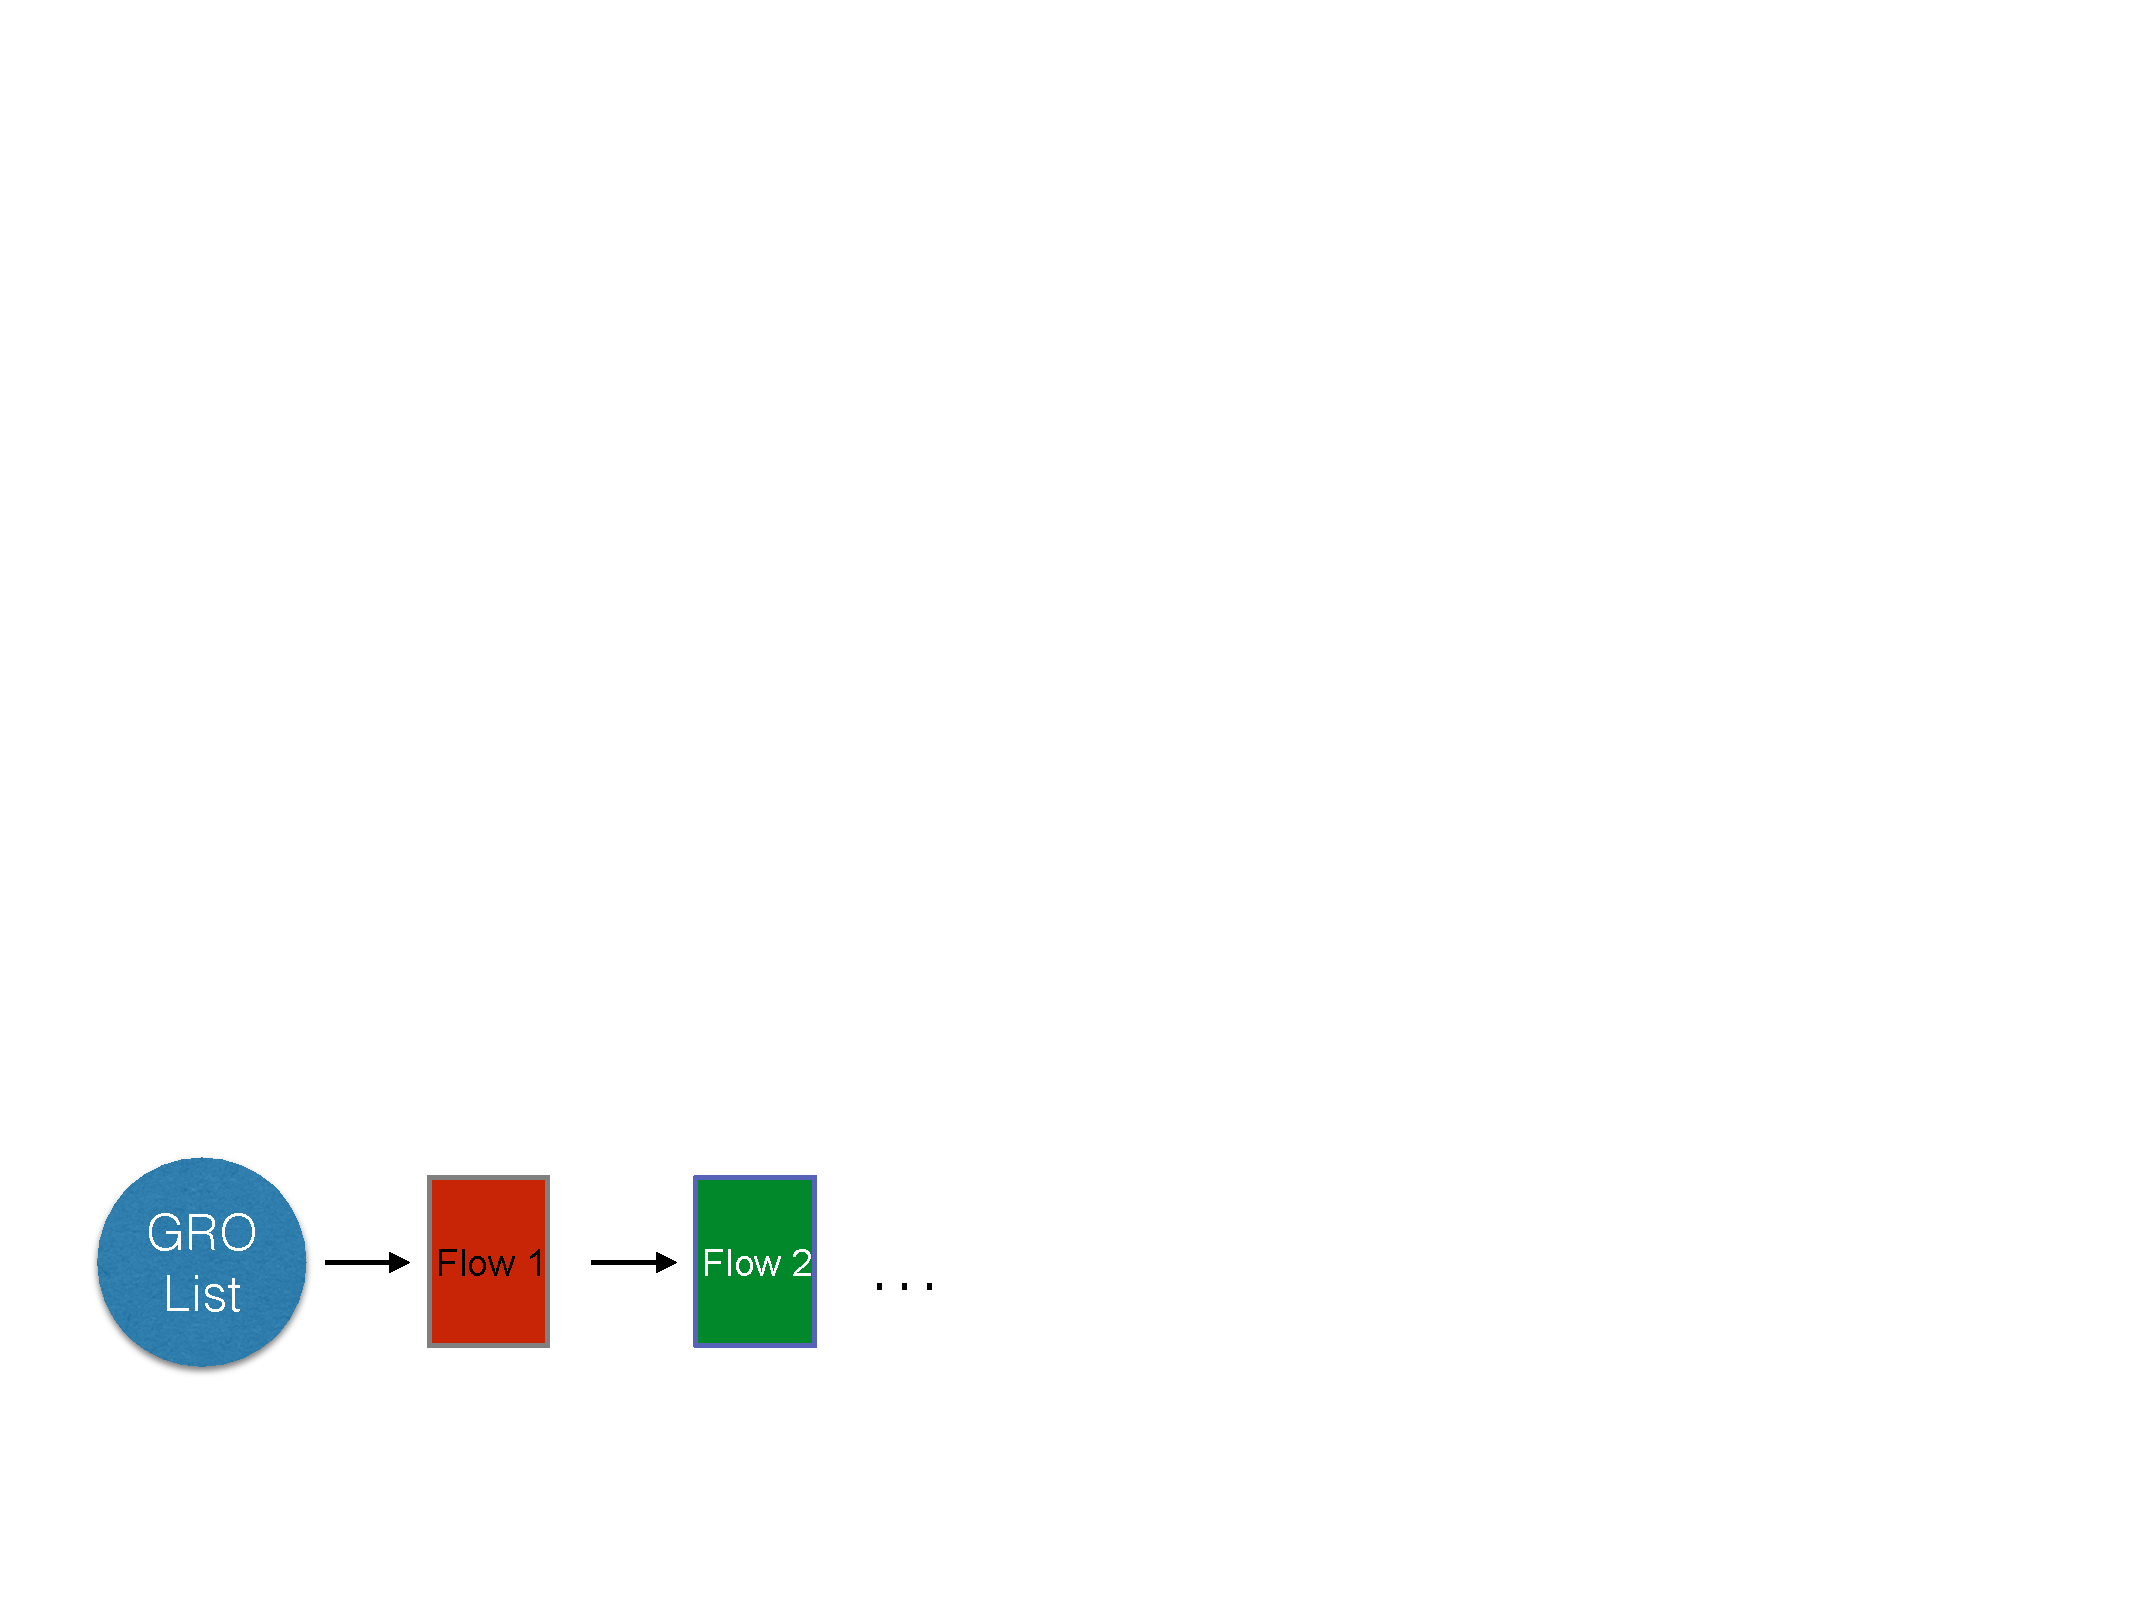
\includegraphics[width=0.45\textwidth]{presto/figures/gro-design/gro.pdf}
%        \caption{GRO design. FIX ME!}
%        \label{gro-design}
%\end{figure}

\begin{figure}[!t]
        \centering
  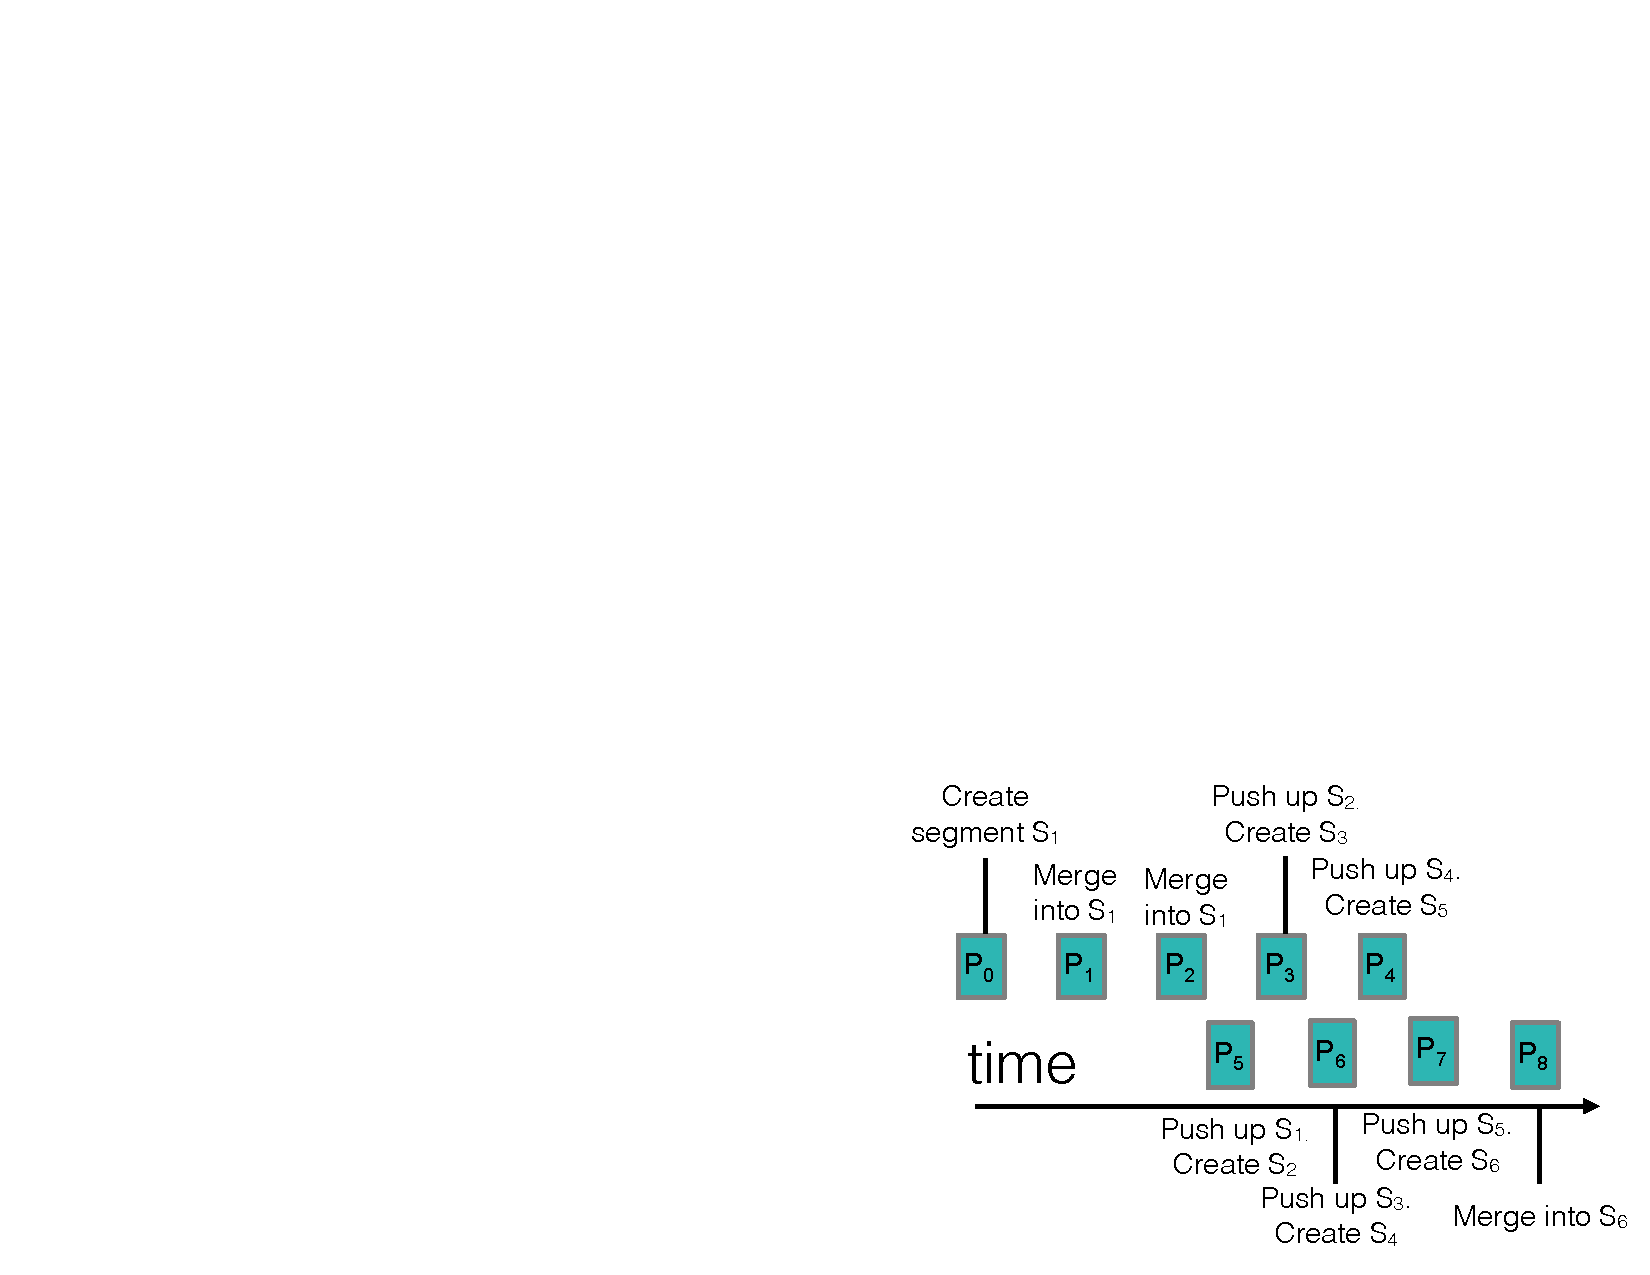
\includegraphics[width=0.7\textwidth]{presto/figures/gro-design/gro-break.pdf}
        \caption{GRO pushes up small segments ($S_i$) during reordering.}
        \label{gro-break}
\end{figure}


We now uncover how GRO breaks down in the face of reordering. Figure~\ref{gro-break} shows the impact of reordering on GRO.  Reordering does not allow the segment to grow: each reordered packet cannot be merged with the existing segment, and thus the previously created segment must be pushed up. With extreme reordering, GRO is effectively disabled because small MTU-sized segments are constantly pushed up. This causes (i) severe computational overhead and (ii) TCP to be exposed to significant amounts of reordering. We term this the {\em small segment flooding} problem.

Determining where to combat the reordering problem has not previously taken the small segment flooding problem into account.  Using a reordering buffer to deal with reordered packets is a common solution (\eg{}works like~\cite{drb} re-sort out-of-order packets in a shim layer below TCP), but a buffer implemented above GRO cannot prevent small segment flooding.  Implementing a buffer below GRO means that the NIC must be changed, which is (i) expensive and cumbersome to update and (ii) unlikely to help combat reordering over multiple interrupts.

In our system, the buffer is implemented in the GRO layer itself.  We argue this is a natural location because GRO can
directly control segment sizes while simultaneously limiting the impact of reordering. 
Furthermore, GRO can still be applied on packets pushed up from LRO, which means hardware doesn't have to be modified
or made complex.
Implementing a better GRO algorithm has multiple challenges. The algorithm should be light-weight to scale to fast networking speeds. Furthermore, an ideal scheme should be able to distinguish loss from reordering.  When a gap in sequence numbers is detected (\eg{}when $P_5$ is received after $P_2$ in Figure~\ref{gro-break}), it is not obvious if this gap is caused from loss or reordering.  If the gap is due to reordering, GRO should not push segments up in order to try to wait to receive the missing gap and merge the missing packets into a preestablished segment.  If the gap is due to loss, however, then GRO should immediately push up the segments to allow TCP to react to the loss as fast as possible. Ideally, an updated GRO algorithm should ensure TCP does not perform any worse than a scheme with no reordering. Finally, the scheme should adapt to prevailing network conditions, traffic patterns and application demands.




\section{Design}
\label{rate-limiter:sec:design}

\subsection{Direct ECE Marking}
\begin{algorithm}[!t]
\caption{Pseudo-code of Direct ECE Marking Algorithm}
\label{alg:algorithm1}
\begin{algorithmic}[1]
\FOR{each incoming TCP ACK p}
\STATE q $\leftarrow$ rate\_limiter\_queue(p)
\IF{len(q) $>$ {\emph {K}}}
\STATE tcp(p).ece $\leftarrow$ 1
\ENDIF
\ENDFOR
\end{algorithmic}
\end{algorithm}

In this subsection, we introduce a technique called Direct ECE Marking (DEM). 
DEM assumes that VMs and containers are configured with DCTCP congestion control algorithm. 
In~\dem{}, we monitor rate limiter queue occupancy and process each incoming TCP ACK. 
If the current rate limiter queue occupancy is above a threshold $K$, 
we directly set the ACK's TCP ECE (ECN Echo) bit to 1.
To get the correct rate limiter queue occupancy for the TCP ACK, we need to inspect the TCP ACK and
determine which queue the incoming TCP ACK's data packet belongs to. In other words, we need to 
determine the queue that this TCP ACK's reverse flow goes to.
The pseudo-code of~\dem{} is presented in Algorithm~\ref{alg:algorithm1}.~\dem{} can be
implemented in the virtual switch (e.g., OVS) in the hypervisor. OVS rate limiters directly call
the Linux HTB implementation so it can get the rate limiter queue information. Also, OVS processes all the packets
so it can inspect and modify all the incoming TCP ACKs. 

The difference between~\dem{} 
and existing ECN marking schemes is that it directly marks TCP ECE bit based on 
current queue occupancy instead of the queue occupancy one TCP RTT ago if using the existing ECN marking schemes.
Therefore, congestion control actions depend on real-time queueing information and control loop latency 
is reduced to almost 0. Control loop latency is the time it takes to forward the TCP ACK from the 
virtual switch to the VM or container. In this way, ``in network'' latency does not cause 
side-effects for end-host congestion control. Note that if we perform ECN marking on the outgoing path, then 
congestion control loop latency can be very large (e.g., RTT of the flows to remote clients is tens of ms).
Besides reducing control loop latency,~\dem{} also avoids coarse-grained segment-level ECN marking, 
which leads to inaccurate congestion level estimation, as we discussed before.
Therefore,~\dem{} makes rate limiter congestion control more timely and effective.

DEM only turns TCP ECE bit from 0 to 1, it never does the opposite. 
If congestion happens both in the rate 
limiter on the end-host and in the switch(es) on the network path, Then TCP ECE bit is always 1. 
If congestion only happens
in the rate limiter, then~\dem{} turns TCP ECE bit from 0 to 1. 
If congestion only happens in the network (i.e., in the switches), then TCP ECE is kept as 1.
If neither network switches nor the rate limiter is congested, then TCP ECE is always 0.
So~\dem{} does not affect the correctness of end-to-end
congestion control and is complementary with ``in network'' congestion control schemes.

\iffalse
\subsection{~\spring{}}

\begin{algorithm}[!t]
\caption{Pseudo-code of~\spring{} Algorithm}
\label{alg:algorithm3}
\begin{algorithmic}[1]
\FOR{each packet p}
\STATE q $\leftarrow$ rate\_limiter\_queue(p)
\STATE current\_qlen $\leftarrow$ len(q)
\STATE new\_gradient $\leftarrow$ current\_qlen -- q.prev\_qlen
\STATE q.prev\_qlen $\leftarrow$ current\_qlen
\STATE q.gradient $\leftarrow$ (1 -- $\alpha$)*q.gradient + $\alpha$*new\_gradient
\STATE q.normalized\_gradient $\leftarrow$ q.gradient / {\emph {K1}}
\IF{p is an incoming TCP ACK}
\STATE f $\leftarrow$ getReverseFlow(p)
\IF {current\_qlen $<$ {\emph {K1}}}
\STATE f.rwnd $\leftarrow$ f.rwnd + MSS
\ELSIF {current\_qlen $>$ {\emph {K2}}}
\STATE f.ssthresh $\leftarrow$ f.rwnd
\STATE f.rwnd $\leftarrow$ f.rwnd*(1 -- $\beta$*(1 -- $\frac{current\_qlen}{K2}$))
\STATE f.rwnd $\leftarrow$ min(f.rwnd, MSS)
\ELSIF {q.gradient $\le$ 0}
\STATE f.rwnd $\leftarrow$ f.rwnd + MSS
\ELSE
\STATE f.rwnd $\leftarrow$ f.rwnd*(1 -- $\beta$*q.normalized\_gradient)
\STATE f.rwnd $\leftarrow$ min(f.rwnd, MSS)
\ENDIF
\ENDIF
\ENDFOR
\end{algorithmic}
\end{algorithm}

DEM has two limitations. First is that it relies on 
DCTCP transport in VMs and containers. For containers, cloud administrators are able to configure
server's congestion control algorithm to DCTCP. So such an assumption is reasonable. 
However, for VMs, tenants have the flexibility to tune their congestion control settings.
Therefore, assuming that every VM uses DCTCP as the congestion control algorithm is not realistic in practice.
Second,~\dem{} needs ECN support in the network. As mentioned before, 
ECN is not widely supported in WAN traffic~\cite{kuhlewind2013state}.
To address the limitations and make our solution more generic, we present~\spring{} (shown in Algorithm~\ref{alg:algorithm3}).

~\spring{} modifies TCP ACK's receiver's 
advertised window size (RWND) to enforce congestion control~\cite{he2016ac,cronkite2016virtualized}.
It uses real-time rate limiter queue length as congestion control signal and 
a TIMELY-like~\cite{mittal2015timely} congestion control law.
For each packet, 
we get its corresponding rate limiter queue length.
If the packet is outgoing, we get the length of the queue that the packet is to be enqueued.
If the packet is an incoming TCP ACK, we get the length of the queue that 
its reverse flow goes to (TCP is bidirectional).  
We maintain a gradient for the rate limiter queue length using 
Exponentially Weighted Moving Average (EWMA) (line 2--6). 
We set two thresholds, $K1$ and $K2$ ($K1 < K2$). The queue length gradient is normalized by dividing it using $K1$ (line 7).
Note that gradient is a per-queue defined parameter.
If the processed packet is an incoming TCP ACK, we first need to get its reverse 
flow (i.e., the TCP ACK's corresponding data packet flow). Then, 
we manage a running RWND for each flow based on a TIMELY-like congestion control law 
(line 10-- line 20). There are 4 cases: 
if the current rate limiter queue length is smaller than $K1$, that means this is no congestion, so we 
increase the flow's RWND by one MSS (Maximum Segment Size). If the current rate limiter queue length is larger
than $K2$, that means congestion happens in the rate limiter queue, so we multiplicatively decrease the RWND. 
If the current rate limiter queue length is between $K1$ and $K2$, we check the gradient of rate limiter queue occupancy.
If the gradient is smaller than or equal to 0, that means the queue is being drained or its size is not increasing, we 
increase RWND by one MSS. Otherwise, we multiplicatively decrease the RWND based on the normalized gradient.

Note that TIMELY~\cite{mittal2015timely} is a rate-based congestion control algorithm while~\spring{} is a window-based.
TIMELY uses accurate latency measurement provided by the NIC while~\spring{} performs congestion control based on 
real-time rate limiter queue length. Because congestion control decisions are enforced via modifying RWND field in TCP ACK headers,~\spring{} has the following good properties: 
1) the solution does not relies on DCTCP transport in VMs and ECN support in the network, 
so it is generic and can support not only east-west traffic (i.e., intra-datacenter traffic) but also north-south traffic
(i.e., inter-datacenter traffic and traffic between cloud and clients). 
2) the solution avoids coarse-grained segment-level ECN marking and its control loop latency is almost 0, so congestion control
is more effective compared with the strawman solution---DCTCP in VMs/containers and ECN marking in rate limiter queues.  

\subsection{Remarks}
Both~\dem{} and~\spring{} avoid long and unpredictable congestion control loop latency and avoid throughput oscillation due to 
coarse-grained segment-level ECN marking.~\dem{} relies on ECN support in the network and DCTCP transports configured in
the end-points. Compared with~\dem{},~\spring{} is a more generic solution.~\dem{} and~\spring{} share the same limitation, that is
they do not support IPSec (because they need to modify TCP header). However, SSL/TLS is supported. 
Furthermore,~\spring{} needs to maintain per-flow information in the hypervisor. 
Maintaining per-flow information in switches is conventionally considered to be challenging.
In~\spring{} we only need to maintain the information of the connections from the VMs/Containers running on the end-host. 
Also, recent advances like OVS ConnTrack~\cite{ovs-conntrack} has made connection tracking on the end-host more effective.

\fi 

\section{Methodology}
\label{sec:method}

\tightparagraph{Implementation}
We implemented Presto in Open vSwitch v2.1.2~\cite{ovs-website} and Linux kernel v3.11.0~\cite{kernel}.
In OVS, we modified 5 files and $\sim$600 lines of code. For GRO, we modified 11 files and $\sim$900 lines of code.
%The GRO handler in Presto is implemented in the kernel (in directory {\tt /net/core/})
%, but there have been discussions
%of moving the GRO handling code into network drivers or to a loadable kernel module. (cite XXX). 
%eric-- the reference above is from 2009, so i think we'll skip this

%other sections probably talk about what we did
%Presto uses chunk size of 32KB/25.6$\mu\text{s}$ (used in combination with TCP small queue~\cite{tsq} which is used for
%reducing latencies on network stack) or 
%64KB/51.2$\mu\text{s}$ (default TCP segment offload size) for 10GbE.



%\subsection{Methodology} 
\tightparagraph{Testbed} We conducted our experiments on a physical
testbed consisting of 16 IBM System x3620 M3 servers with 6-core Intel Xeon
2.53GHz CPUs, 60GB memory, and Mellanox ConnectX-2 EN 10GbE NICs. 
The servers were connected in a 2-tier Clos network topology with 10 Gbps
IBM RackSwitch G8264 switches, as shown in Figure~\ref{macro_evaluation_topology}.

\tightparagraph{Experiment Settings}
We ran the default TCP implementation in the Linux kernel (TCP CUBIC~\cite{cubic})
%3.11.0 and uses MPTCP version 0.88~\cite{mptcp-linux}.
%We use default TSO size 64KB
and set parameters {\tt tcp\_sack}, {\tt tcp\_fack}, {\tt tcp\_low\_latency} to 1. 
Further, we tuned the host Receive Side Scaling (RSS)~\cite{rss} and IRQ affinity settings and kept them the same in all experiments.
We send and receive packets from the hypervisor OS instead of VMs. 
LRO is not enabled on our NICs.
%For MPTCP, we set the subflow count to 8, use OLIA congestion control algorithm~\cite{mptcp-not-optimal}, and configure buffer sizes
%as recommended by ~\cite{dc-mptcp,mptcp-not-optimal,paasch2013benefits}.

\tightparagraph{Workloads}
We evaluate Presto with a set of synthetic and realistic workloads. 
Similar to previous works~\cite{fattree,hedera,planck}, our synthetic workloads include:
{\em Shuffle}: Each server in the testbed sends 1GB data to every other server in the testbed in random order. 
Each host sends two flows at a time. %The shuffle is finished if all the servers have finished their jobs. 
This workload emulates the shuffle behavior of Hadoop workloads.
{\em Stride(8)}: We index the servers in the testbed from left to right. In stride(8) workload, server[i] sends to server[(i+8) mod 16].
{\em Random}: Each server sends to a random destination 
 not in the same pod as itself. Multiple senders can send to the same receiver.
{\em Random Bijection}: Each server sends to a random destination not in the same pod as itself. 
Different from random, each server only receives data from one sender.
Finally, we also evaluate Presto with trace-driven workloads from real datacenter traffic~\cite{kandula2009nature}.

\tightparagraph{Performance Evaluation}
We compare Presto to ECMP, MPTCP, and a 
single non-blocking switch used to represent an optimal scenario.
ECMP is implemented by enumerating all possible end-to-end paths and randomly selecting a path for each flow.
MPTCP uses ECMP to determine the paths of each of its sub-flows.
%We use MPTCP version 0.88~\cite{mptcp-linux}, set the subflow count to 8, use OLIA congestion control algorithm~\cite{mptcp-not-optimal}, and configure buffer sizes
%as recommended by ~\cite{dc-mptcp,mptcp-not-optimal,paasch2013benefits}. 
The MPTCP implementation is still under active development, and
we spent significant effort in finding the most stable configuration of MPTCP on our testbed. Ultimately, we found that Mellanox {\tt mlx\_en4} driver version
2.2, MPTCP version 0.88~\cite{mptcp-linux}, subflow count set to 8, OLIA congestion control algorithm~\cite{mptcp-not-optimal}, and configured buffer sizes
as recommended by~\cite{dc-mptcp,mptcp-not-optimal,paasch2013benefits} gave us the best trade-offs in terms of throughput, latency, loss and stability.
Unfortunately, despite our efforts, we still occasionally witness some stability issues 
with MPTCP that we believe are due to implementation bugs.

We evaluate Presto on various performance metrics, including: 
throughput (measured by {\tt nuttcp}), round trip time (a single TCP packet, measured by {\tt sockperf}~\cite{sockperf}), 
mice flow completion time (time to send a 50 KB flow and receive an application-layer acknowledgement), packet loss (measured from switch counters), 
and fairness (Jain's fairness index~\cite{jain-fair} over flow throughputs).  Mice flows are sent every 100 ms and elephant flows last 10 seconds. 
Each experiment is run for 10 seconds over 20 runs. Error bars on graphs denote
the highest and lowest value over all runs.


\section{Microbenchmarks}
\label{sec:micro}

We first evaluate the effectiveness of Presto over a series of microbenchmarks: %. Using 
%canonical topologies, we investigate 
(i) Presto's effectiveness in preventing the small segment
flooding problem and reordering, (ii) Presto's CPU overhead, (iii) Presto's ability to scale
to multiple paths, (iv) Presto's ability to handle congestion, (v) comparison to flowlet
switching, and (vi) comparison to local, per-hop load balancing.

%%%%%micro test - scalability and congestion test topology
\begin{figure}[!t]
        \centering
	\begin{subfigure}[b]{0.45\textwidth}
        	\centering
  		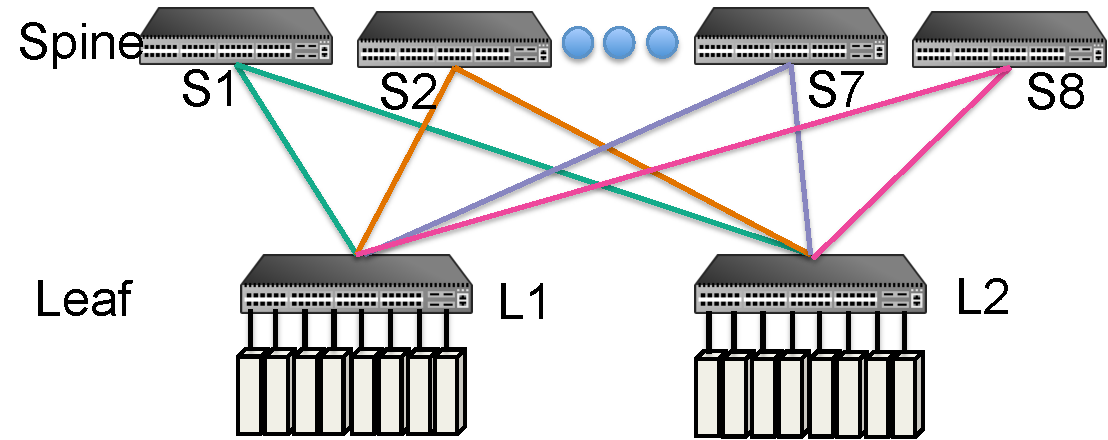
\includegraphics[width=\textwidth]{presto/figures/micro_test_topology/micro_scalabilitytest_topology_refined.pdf}
        	\caption{}
		\label{micro_scalability_topology}
	\end{subfigure}
	\begin{subfigure}[b]{0.45\textwidth}
                \centering
		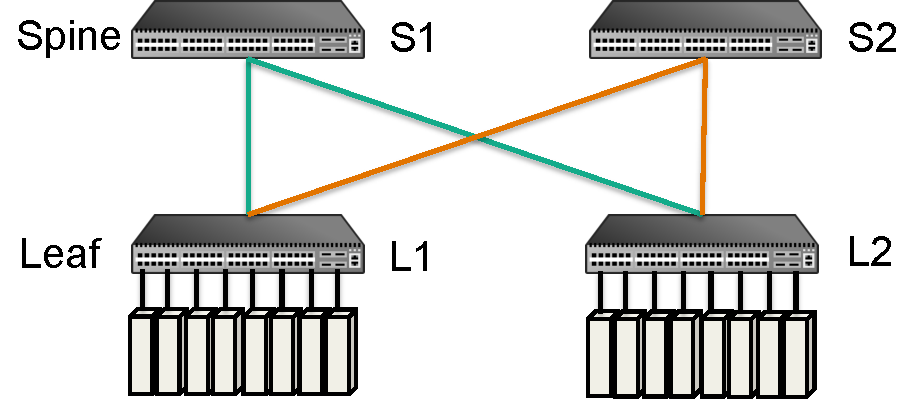
\includegraphics[width=\textwidth]{presto/figures/micro_test_topology/micro_congestiontest_topology_refined.pdf}
        	\caption{}
		\label{micro_congestion_topology}
	\end{subfigure}
	\caption{(a) Scalability benchmark and (b) Oversubscription benchmark topology.}
	\label{micro_topology}
\end{figure}

%%%%%gro effectiveness shows
\begin{figure}[!t]
	\centering
	\begin{subfigure}[b]{0.45\textwidth}
                \centering
  		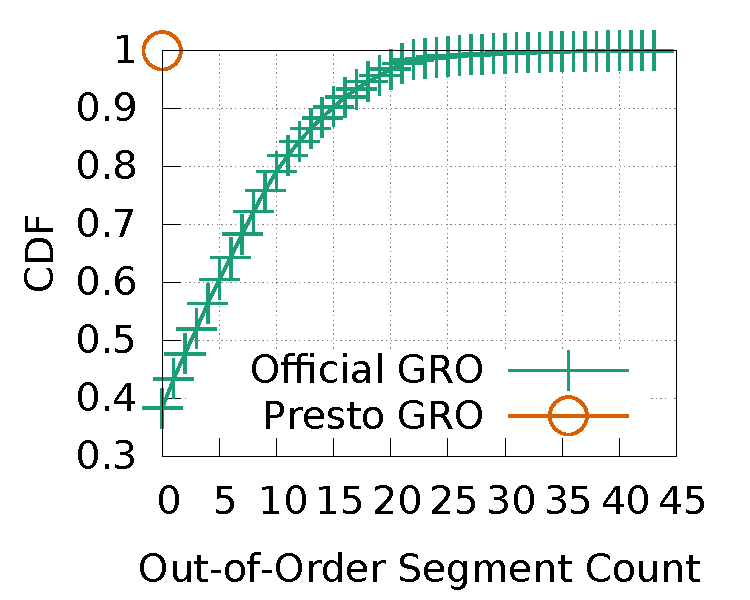
\includegraphics[width=\textwidth]{presto/figures/gro_effectiveness/metric1_seg_cdf_compare.pdf}
		\caption{}
		\label{gro_effectiveness_on_reordering}
	\end{subfigure}
        \begin{subfigure}[b]{0.45\textwidth}
                \centering
		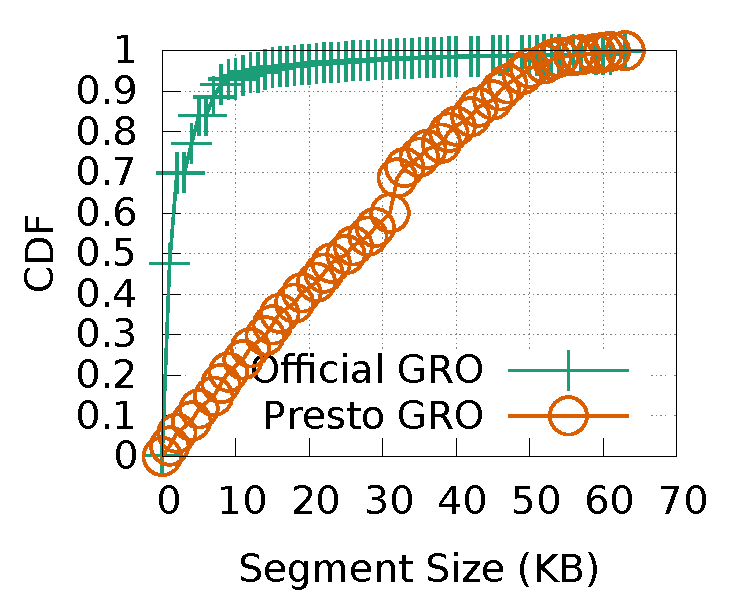
\includegraphics[width=\textwidth]{presto/figures/gro_effectiveness/metric1_pktsize_cdf_compare.pdf}
        	\caption{}
		\label{gro_effectiveness_on_pktsize}
	\end{subfigure}
	\caption{(a) Illustration of the modified GRO's effectiveness on masking reordering. 
		%We use the number of  segments from other chunks
                %between the first segment and last segment of each chunk
                %seen by TCP to measure the extent of packet reordering
		(b) In case of massive packet reordering, official GRO cannot merge packets effectively such that lots of small
                packets are processed by TCP which poses great processing overhead for CPU.}
	\label{gro_effectiveness}
\end{figure}

\tightparagraph{Presto's GRO Combats Reordering}
To examine Presto's ability to handle packet reordering, we perform a simple experiment
on the topology shown in Figure~\ref{micro_congestion_topology}.
%we compare the extent of TCP reordering, TCP segment size distribution, throughput and receiver side CPU usage 
%using official GRO and Presto GRO. 
Here two servers attached to leaf switch L1 
send traffic to their own receivers attached to leaf switch L2
by spreading flowcells over two network paths. 
%Because these two flows share the same two paths 
%so packet reordering can happen at the receiver side.
This setup can cause reordering for each flow, so 
we compare Presto's GRO to
an unmodified GRO, denoted "Official GRO". 
The amount of reordering exposed to TCP is presented in Figure~\ref{gro_effectiveness_on_reordering}.
To quantify packet reordering, we show a CDF of the {\em out-of-order segment count}: ~\ie{},
the number of segments from other flowcells between the first packet and last packet of each flowcell. A value of zero
means there is no reordering and larger values mean more reordering. The figure shows Presto's GRO can completely mask reordering
while official GRO incurs significant reordering. As shown in Section~\ref{sec:background}, reordering can
also cause smaller segments to be pushed up the networking stack, causing significant processing overhead.
Figure~\ref{gro_effectiveness_on_pktsize} shows the received TCP segment size distribution.  Presto's GRO
pushes up large segments, while the official GRO pushes up many small segments.
The average TCP throughputs in official GRO and Presto GRO are 4.6 Gbps (with 86\% CPU utilization) and 
9.3 Gbps (with 69\% CPU utilization), respectively. Despite the fact that official GRO only obtains 
about half the throughput of Presto's GRO, it still incurs more than 24\% higher CPU overhead. 
Therefore, an effective scheme must deal with both reordering and small segment overhead.
%\eric{interesting that stride on big testbed w/ official GRO had same numbers: 4.6 Gbps and similar overhead}

\begin{figure}[!t]
        \centering
  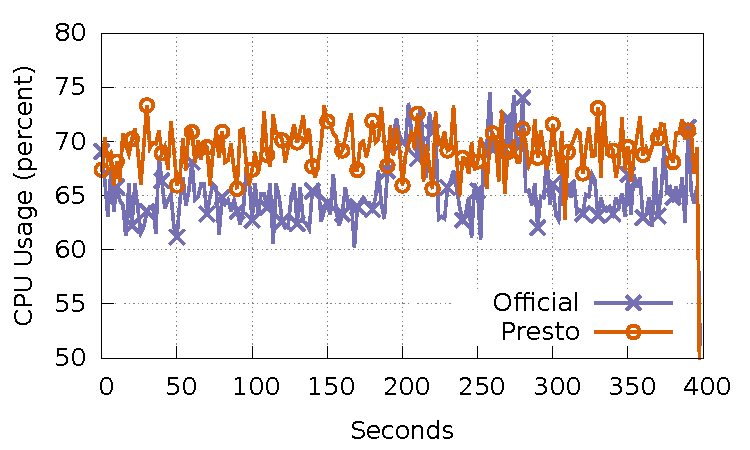
\includegraphics[width=0.7\textwidth]{presto/figures/mornitor_cpu/macro_compare_cpu_usage.pdf}
        \caption{Presto incurs 6\% CPU overhead on average.}
        \label{micro_compare_cpu}
\end{figure}

\tightparagraph{Presto Imposes Limited CPU Overhead}
We investigate Presto's CPU usage by
running the stride workload on a 2-tier Clos network as shown in Figure~\ref{macro_evaluation_topology}. 
For comparison, official GRO is run with the stride workload using a non-blocking switch (so there
is no reordering). Note both official GRO and Presto GRO can achieve 9.3 Gbps.  
The receiver CPU usage is sampled every 2 seconds over a 400 second interval, and
the time-series is shown in Figure~\ref{micro_compare_cpu}. 
%implying that the network utilization is 93% in both cases. 
On average, Presto GRO only increases CPU usage by 6\% compared with the official GRO. 
The minimal CPU overhead comes from Presto's careful design and implementation. 
At the sender, Presto needs just two {\tt memcpy} operations (1 for shadow MAC rewriting, 1 for flowcell ID encoding). 
At the receiver, Presto needs one {\tt memcpy} to rewrite the shadow MAC back to the real MAC and
also incurs slight overhead because multiple segments are now kept per flow. The overhead
of the latter is reduced because these segments are largely kept in reverse sorted order, which means {\tt merge}
on an incoming packet is usually $\mathcal{O}(1)$. The insertion sort is done at the beginning of each {\tt flush} event over a small
number of mostly in-order segments, which amortizes overhead because it is called infrequently compared to {\tt merge}.

%%%%%scalability test figures %%%%
\begin{figure}[!t]
        \centering
  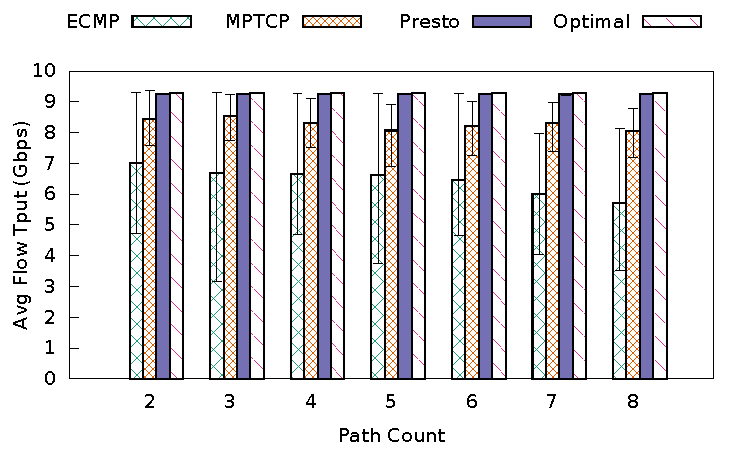
\includegraphics[width=0.7\textwidth]{presto/figures/scalability_test/scalability_compare_tput_witherrbar.pdf}
        \caption{Throughput comparison in scalability benchmark. We denote the non-blocking case as Optimal. 
		} 
        \label{micro_scalability_test_tput}
\end{figure}

%merged with scalability loss rate
\iffalse
\begin{figure}[ht]
        \centering
  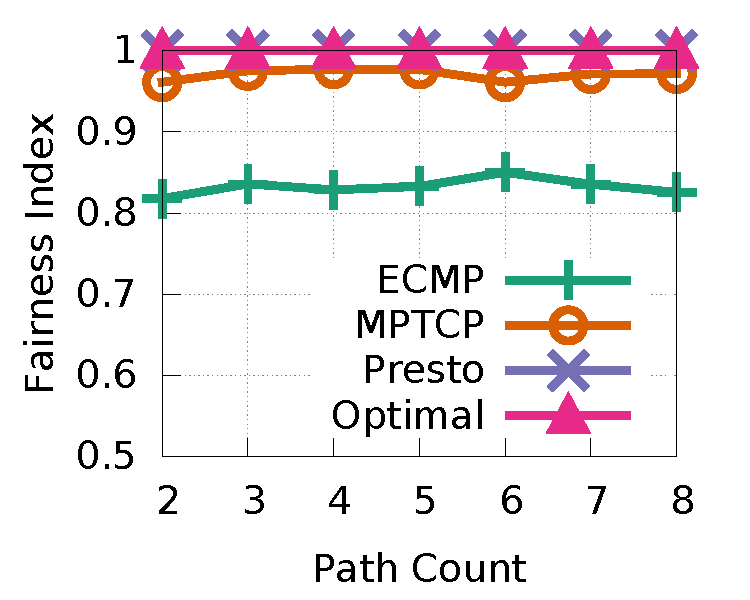
\includegraphics[width=0.45\textwidth]{presto/figures/scalability_test/scalability_compare_fairness.pdf}
        \caption{Micro benckmark 2 - scalability test. 
		We increase the number of spine switches (i.e., the number of intermediate paths)
                and set the number of flows (host pairs) equal to the number of available paths. 
		Fairness comparison. 20 runs each with each run lasting for 10 seconds.
		Optimal means running TCP on a non-blocking network}
        \label{micro_scalability_test_fairness}
\end{figure}
\fi

\begin{figure}[!t]
        \centering
  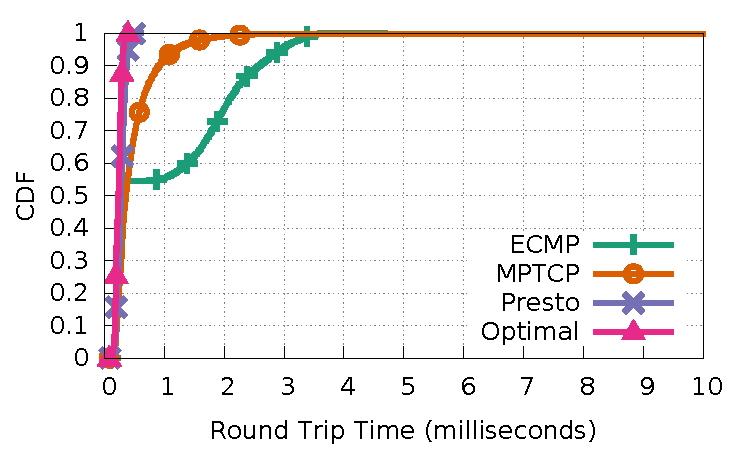
\includegraphics[width=0.7\textwidth]{presto/figures/scalability_test/scalability_compare_latency.pdf}
        \caption{Round trip time comparison in scalability benchmark. 
		%We increase the number of spine switches (i.e., the number of intermediate paths)
                %and set the number of flows (host pairs) equal to the number of available paths. 
		}
        \label{micro_scalability_test_latency}
\end{figure}


\begin{figure}[!t]
        \centering
	\centering
        \begin{subfigure}[b]{0.45\textwidth}
                \centering
		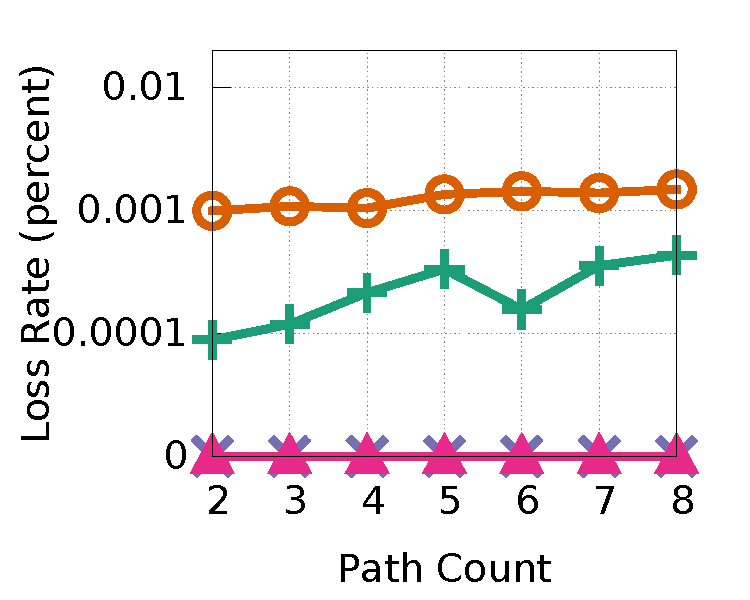
\includegraphics[width=\textwidth]{presto/figures/scalability_test/scalability_compare_loss.pdf}
		\caption{}
		\label{micro_scalability_test_loss}
        \end{subfigure}
        \begin{subfigure}[b]{0.45\textwidth}
  		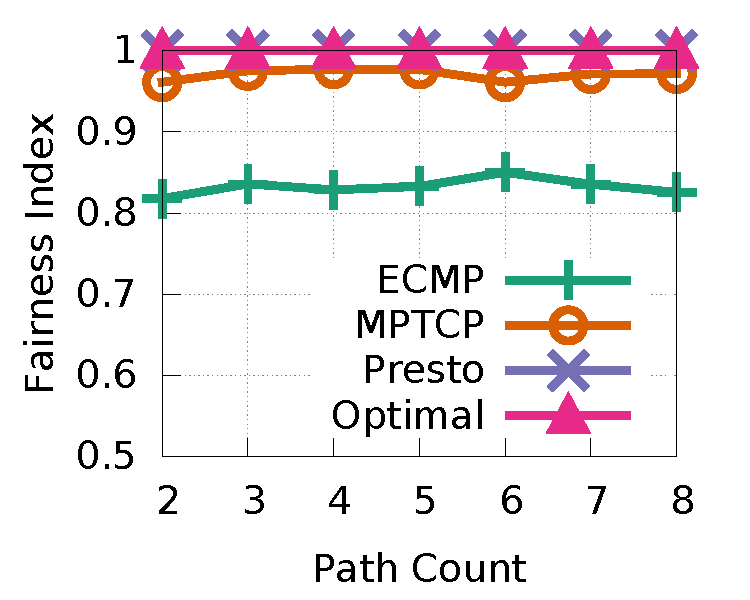
\includegraphics[width=\textwidth]{presto/figures/scalability_test/scalability_compare_fairness.pdf}
        	\caption{}
        	\label{micro_scalability_test_fairness}
	\end{subfigure}
	\caption{(a) Loss rate and (b) Fairness index comparison in scalability benchmark.}
\end{figure}

\tightparagraph{Presto Scales to Multiple Paths}
We analyze Presto's ability to scale in the number of paths by
setting the number of flows (host pairs) equal to the number of available paths in the topology shown in 
Figure~\ref{micro_scalability_topology}. The number of paths is varied from 2 to 8, and 
Presto always load-balances over all available paths.
Figure~\ref{micro_scalability_test_tput} shows Presto's throughput closely tracks Optimal. 
ECMP (and MPTCP) suffer from lower throughput when flows (or subflows) are
hashed to the same path. Hashing on the same path leads to congestion and thus increased latency, as shown in Figure~\ref{micro_scalability_test_latency}.
Because this topology is non-blocking and Presto load-balances in a near optimal fashion, Presto's latency
is near Optimal. Packet drop rates are presented in Figure~\ref{micro_scalability_test_loss} and show
Presto and Optimal have no loss. MPTCP has higher loss because of its bursty nature~\cite{conga}
and its aggression in the face of loss: when a single loss occurs, only
one subflow reduces its rate. The other schemes are more conservative because a single loss reduces the rate of the whole flow.
Finally, Figure~\ref{micro_scalability_test_fairness} shows Presto, Optimal and MPTCP
achieve almost perfect fairness.
%The underlying reason is that MPTCP makes traffic more bursty~\cite{conga}.


%%%congestion test figures %%%%
\begin{figure}[!t]
        \centering
  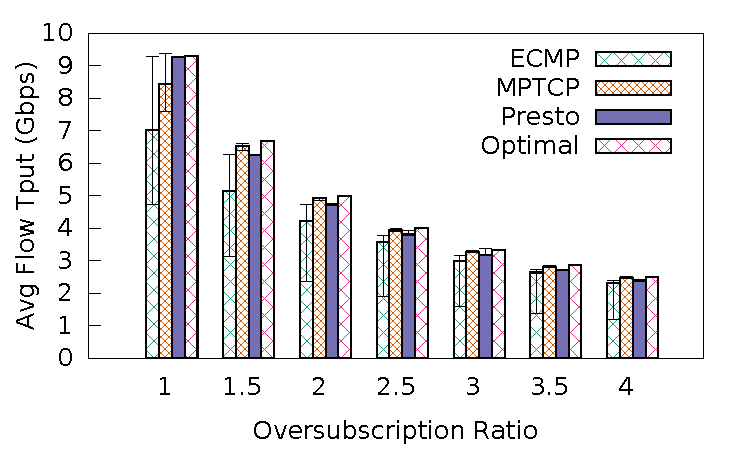
\includegraphics[width=0.7\textwidth]{presto/figures/congestion_test/congestion_compare_tput_witherrbar.pdf}
        \caption{Throughput comparison in oversubscription benchmark.}
        \label{micro_congestion_test_tput}
\end{figure}


\begin{figure}[!t]
        \centering
  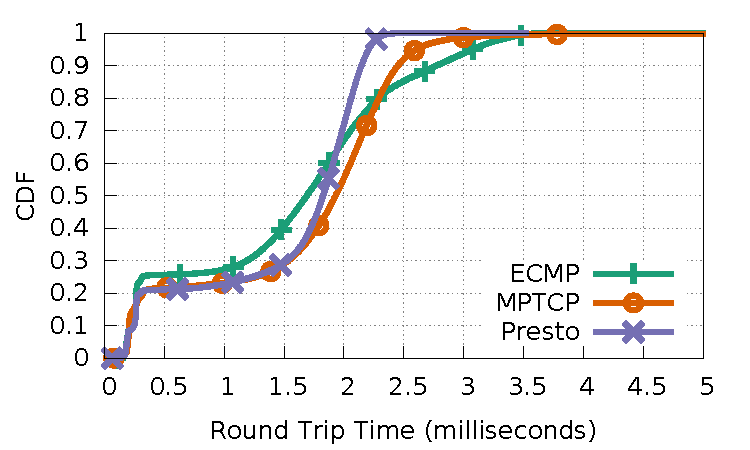
\includegraphics[width=0.7\textwidth]{presto/figures/congestion_test/congestion_compare_latency.pdf}
        \caption{Round trip time comparison in oversubscription benchmark.
		}
        \label{micro_congestion_test_latency}
\end{figure}



\begin{figure}[!t]
        \centering
	\centering
        \begin{subfigure}[b]{0.45\textwidth}
                \centering
		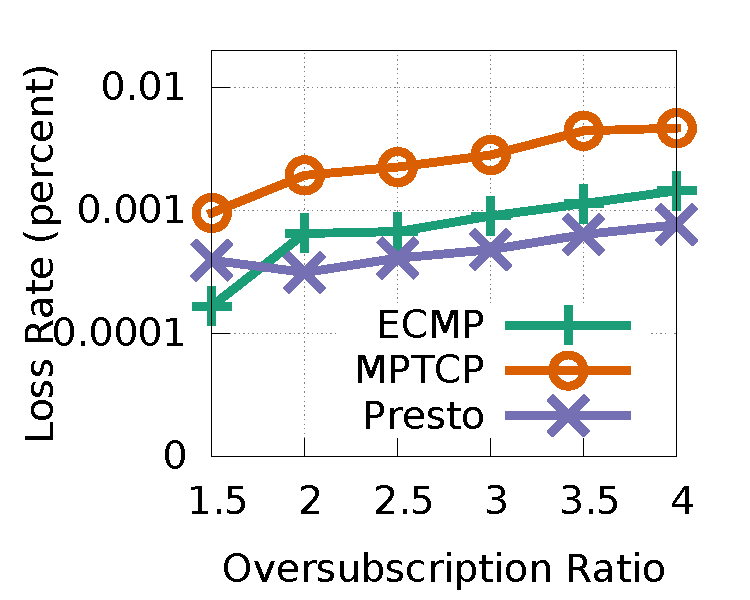
\includegraphics[width=\textwidth]{presto/figures/congestion_test/congestion_compare_loss.pdf}
		\caption{}
		\label{micro_congestion_test_loss}
	\end{subfigure}
	\begin{subfigure}[b]{0.45\textwidth}
		\centering
  		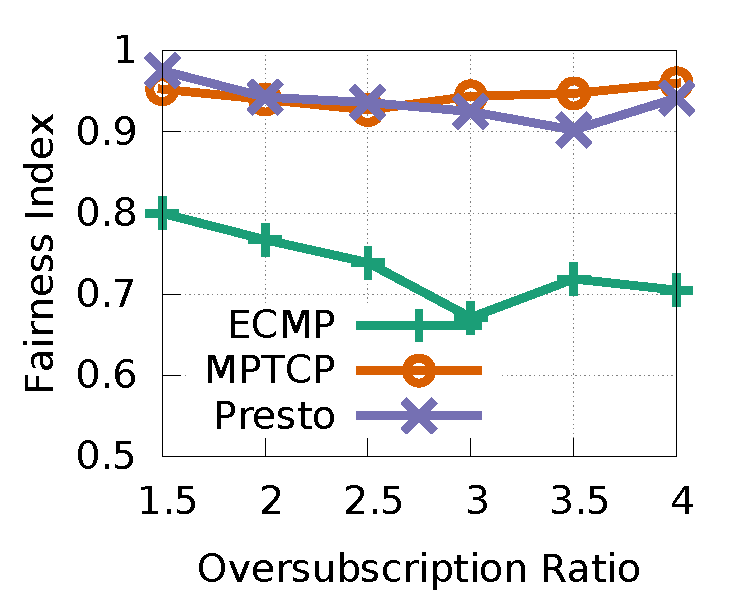
\includegraphics[width=\textwidth]{presto/figures/congestion_test/congestion_compare_fairness.pdf}
		\caption{}
        \label{micro_congestion_test_fairness}
	\end{subfigure}
	\caption{(a) Loss rate and (b) Fairness index comparison in oversubscription benchmark.}
\end{figure}

\tightparagraph{Presto Handles Congestion Gracefully}
Presto's ability to handle congestion is analyzed by fixing 
the number of spine and leaf switches to 2 and varying
the number of flows (host pairs) from 2 to 8, as shown
in Figure~\ref{micro_congestion_topology}. 
Each flow sends as much as possible, which leads to the network
being oversubscribed by a ratio of 1 (two flows) to 4 (eight flows).
Figure~\ref{micro_congestion_test_tput} shows all schemes track Optimal in highly
oversubscribed environments. ECMP
does poorly under moderate congestion because the limited number of flows can be hashed to the same path.
Presto does no worse in terms of latency (Figure~\ref{micro_congestion_test_latency}) and loss (Figure~\ref{micro_congestion_test_loss}).
The long tail latency for MPTCP is caused by its higher loss rates.
Both Presto and MPTCP have greatly improved fairness compared with ECMP (Figure~\ref{micro_congestion_test_fairness}).

\begin{figure}[!t]
        \centering
  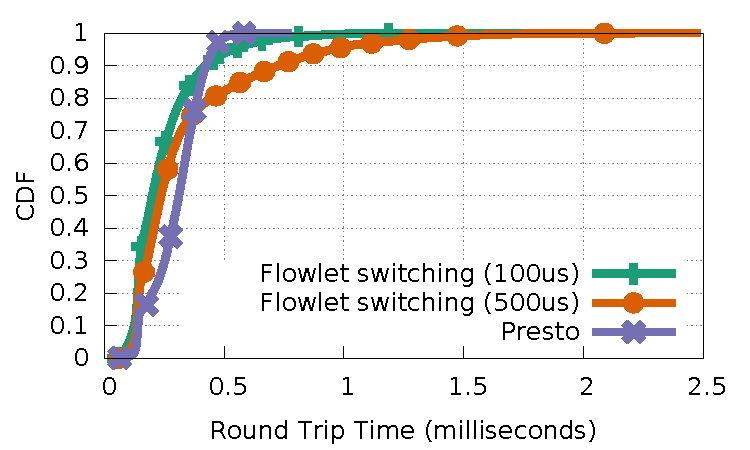
\includegraphics[width=0.7\textwidth]{presto/figures/flowlets/flowlet_switching/flowlet_presto_compare_sockperf.pdf}
        \caption{Round trip time comparison of flowlet switching and Presto in Stride workload. 
		The throughputs of Flowlet switching with 100 $\mu\text{s}$ gap, 500 $\mu\text{s}$ gap and Presto 
		are 4.3 Gbps, 7.6 Gbps and 9.3 Gbps respectively. }
        \label{micro_flowlet_rtt_compare}
\end{figure}


\tightparagraph{Comparison to Flowlet Switching}
We first implemented a flowlet load-balancing scheme in OVS that detects
inactivity gaps and then schedules flowlets over disjoint paths in a round robin fashion.
%(Presto does this over flowcells instead of flowlets).
The receiver for flowlets uses official GRO.
Our flowlet scheme is not a direct reflection of CONGA because (i) it is not 
congestion-aware and (ii) the flowlets are determined in the software edge
instead of the networking hardware.
Presto is compared to 500 $\mu$s and 100 $\mu$s inactivity timers in
the stride workload on the 2-tier Clos network (Figure~\ref{macro_evaluation_topology}).
The throughput of the schemes are 9.3 Gbps (Presto), 7.6 Gbps (500 $\mu$s), and 4.3 Gbps (100 $\mu$s).
%Switching flowlets on very small timescales, such as 100$\mu$s, provides opportunities to create many flowlets.
%The largest flowlet is only 0.20\% (XX) of the total network traffic, which corresponds to about 5-9 MB in our runs.
%And while small flowlets create an even distribution
%of traffic over the network, significant strain is put on the TCP connection due to packet reordering. 
Analysis of the 100 $\mu$s
network traces show 13\%-29\% packets in the connection are reordered, which means 100 $\mu$s is not enough
time to allow packets to arrive in-order at the destination and thus throughput is severely impacted. Switching flowlets with 500 $\mu$s prevents
most reordering (only 0.03\%-0.5\% packets are reordered), but creates very large flowlets (see Figure~\ref{micro_flowlet_size}). This means
flowlets can still suffer from collisions, which can hurt throughput (note: while not shown here, 500 $\mu$s outperforms ECMP by over 40\%).
Figure~\ref{micro_flowlet_rtt_compare} shows the
latencies. Flowlet 100 $\mu$s has low throughput and hence lower latencies. However, since
its load balancing isn't perfect, it can still cause increased congestion in the tail. Flowlet 500 $\mu$s
also has larger tail latencies because of more pronounced flowlet collisions. As compared to the flowlet
schemes, Presto decreases 99.9$^{th}$ percentile latency by 2x-3.6x.
%Presto, by enforcing small flowlet sizes and explicitly accounting for reordering on the receiver, can obtain near
%line rate throughput with minimal tail latencies. 



%%%%presto 2 mods (ecmp and shaodw MAC) compare
\begin{figure}[!t]
        \centering
  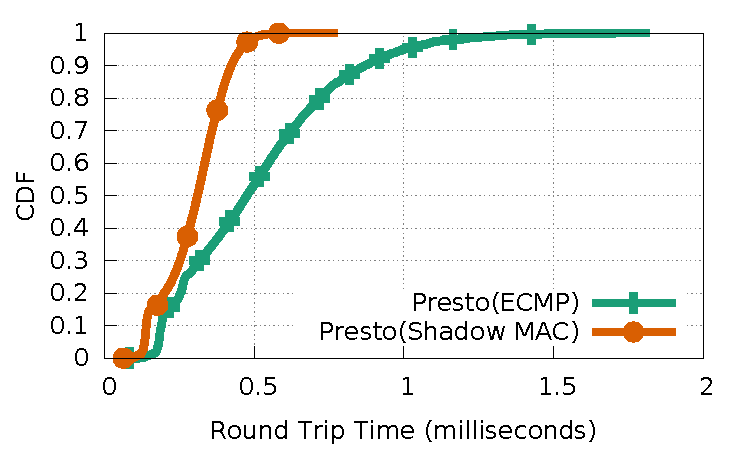
\includegraphics[width=0.7\textwidth]{presto/figures/presto_compare_2modes/presto_compare_2mods.pdf}
        \caption{Round trip time comparison between Presto + shadow MAC and Presto + ECMP.
		%Compare Presto 2 modes' (Presto over ECMP and Presto over Shadow MAC) performance.
                %Simple 2-tier Clos network with 4 senders and 4 receivers, 4 paths between any host pair.
                %10 seconds per run, 20 runs. Use {\tt nuttcp} to measure throughput. Use {\tt sockperf}
                %to measure latency (RTT).
                %In Presto+ECMP, the average throughput is 7.9 (8.7 if trade latency for tput)
                %Gbps while in Presto+Shadow MAC, the
                %average throughput is 9.3Gbps 
		}
        \label{micro_presto_2mods}
\end{figure}

\tightparagraph{Comparison to Local, Per-Hop Load Balancing}
Presto sends flowcells in a round robin fashion over pre-configured end-to-end paths. An alternative is to
have ECMP hash on flowcell ID and thus provide per-hop load balancing. 
%One way to implement Presto + ECMP is to let vSwitch copy real TCP source port into a pre-allocated TCP option field 
%(\todo{this requires TCP stack allocates the new TCP option before sending to vSwitch}) and 
%encode chunk ID into TCP source port field. Because chunk ID is incremental, ECMP randomly maps chunks into multiple paths. 
We compare Presto + shadow MAC with Presto + ECMP using a stride workload on our testbed. 
Presto + shadow MAC's average throughput is 9.3 Gbps while Presto + ECMP's is 8.9 Gbps.
The round trip time CDF is shown in Figure~\ref{micro_presto_2mods}. 
Presto + shadow MAC gives better latency performance compared with Presto + ECMP. 
The performance difference comes from the fact that Presto + shadow MAC provides 
better fine-grained flowcell load balancing because 
randomization in per-hop multipathing can lead to corner cases where
a large fraction of flowcells get sent to the same link over a small timescale by multiple flows. This transient congestion
can lead to increased buffer occupancy and higher delays.

\section{Evaluation}
\label{sec:eval}

%~\todo{needs to go through the text and make sure they are consistent with the figures!!!}
In this section, we analyze the performance of Presto for (i) synthetic workloads, (ii)
trace-driven workloads, (iii) workloads containing north-south cross traffic, and (iv) failures.
All tests are run on the topology in Figure~\ref{macro_evaluation_topology}.
\begin{figure}[!t]
        \centering
  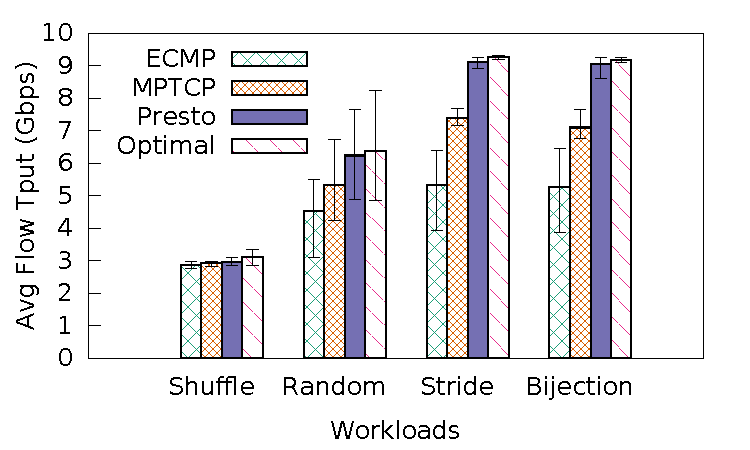
\includegraphics[width=0.7\textwidth]{presto/figures/macro/stride/macro_compare_tput_witherrbar.pdf}
        \caption{Elephant flow throughput for ECMP, MPTCP, Presto and Optimal in shuffle, random, stride and random bijection workloads.}
        \label{macro_evaluation_tput}
\end{figure}



\begin{figure*}[!t]
        \centering
	\begin{subfigure}[b]{0.45\textwidth}
                \centering
  		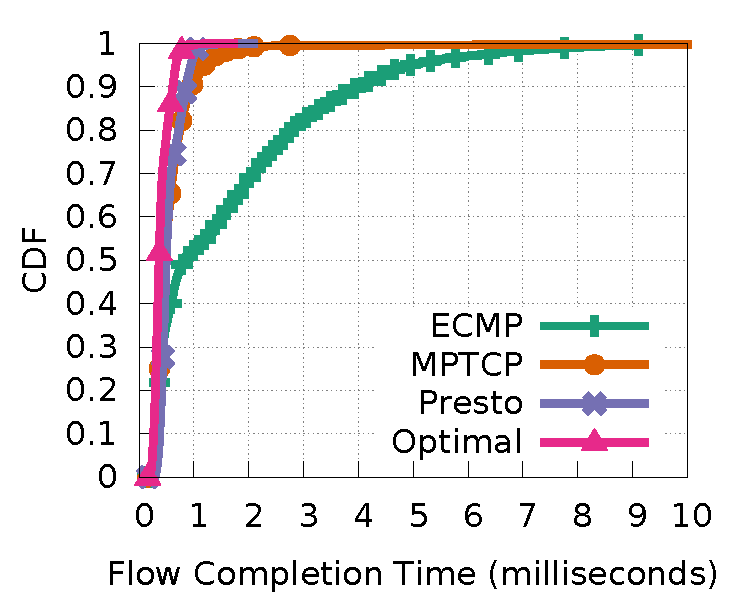
\includegraphics[width=\textwidth]{presto/figures/macro/stride/macro_compare_fct_stride_mice.pdf}
        	\caption{Stride}
        	\label{macro_evaluation_fct_stride}
	\end{subfigure}
	\begin{subfigure}[b]{0.45\textwidth}
                \centering
		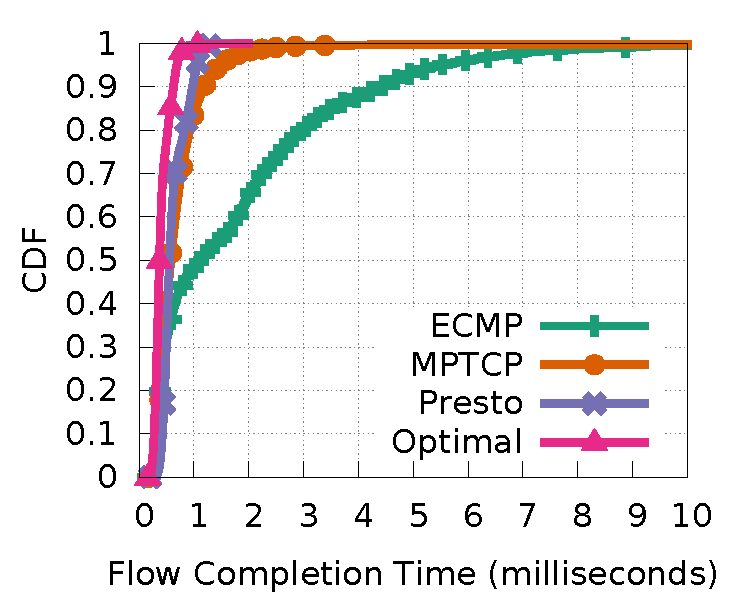
\includegraphics[width=\textwidth]{presto/figures/macro/bijection/macro_compare_fct_bijection_mice.pdf}
        	\caption{Random Bijection}
        	\label{macro_evaluation_fct_bijection}
	\end{subfigure}
        %\begin{subfigure}[b]{0.225\textwidth}
        %        \centering
	%	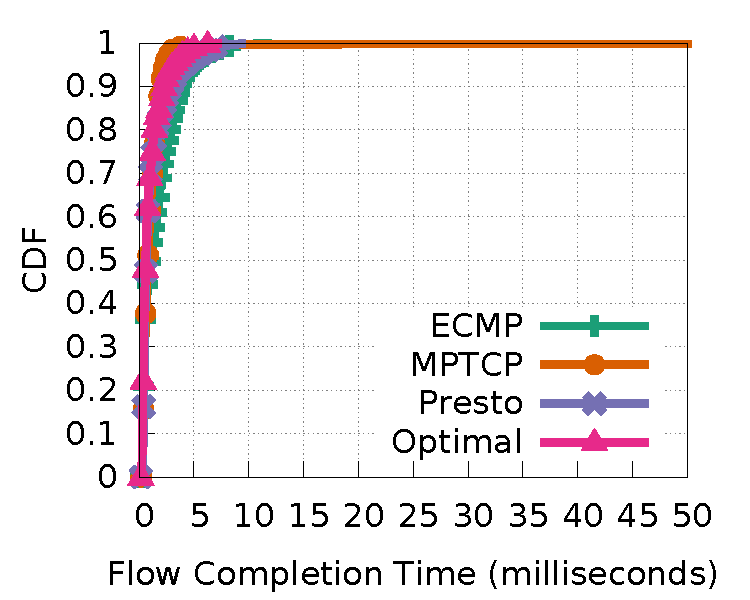
\includegraphics[width=\textwidth]{presto/figures/macro/random/macro_compare_fct_random_mice.pdf}
        %	\caption{Random}
        %	\label{macro_evaluation_fct_random}
	%\end{subfigure}
        \begin{subfigure}[b]{0.45\textwidth}
                \centering
		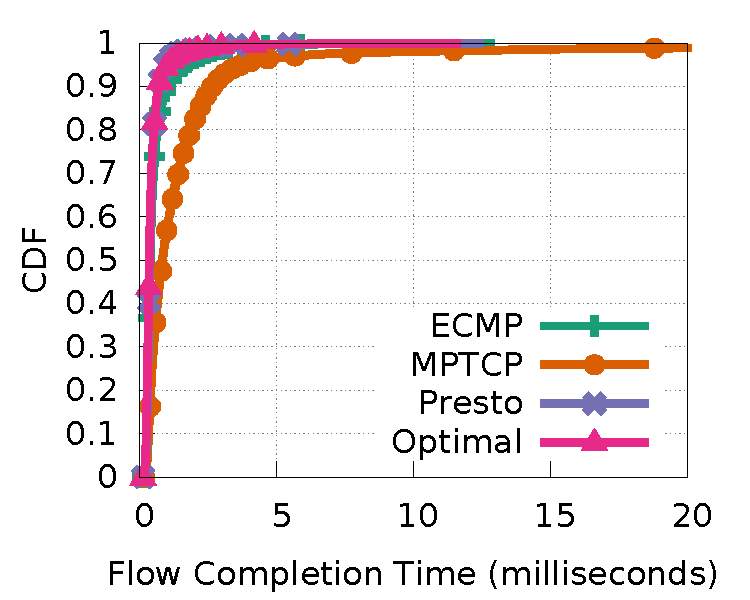
\includegraphics[width=\textwidth]{presto/figures/macro/shuffle/macro_compare_fct_shuffle_mice.pdf}
        	\caption{Shuffle}
        	\label{macro_evaluation_fct_shuffle}
	\end{subfigure}
	\caption{Mice FCT of ECMP, MPTCP, Presto and Optimal in stride, random bijection, and shuffle workloads.}
	\label{macro_evaluation_fct}
\end{figure*}

\tightparagraph{Synthetic Workloads}
Figure~\ref{macro_evaluation_tput} 
shows the average throughputs of elephant flows in the shuffle, random, stride and random bijection workloads.
Presto's throughput is within 1-4\% of Optimal over all workloads.
For the shuffle workload, ECMP, MPTCP, Presto and Optimal show similar results 
because the throughput is mainly bottlenecked at the receiver. 
%due to several servers sending to the same receiver.
In the non-shuffle workloads, Presto improves upon ECMP by 38-72\% and improves
upon MPTCP by 17-28\%.
%Compared with ECMP, 
%Presto improves throughput by 71\% (stride), 72\% (random bijection) and 38\% (random).
%Presto also outperforms MPTCP with throughput improvements of 23\% (stride), 28\% (random bijection) and 
%17\% (random).
%In all the workloads, Presto's throughput outperforms MPTCP.

Figure~\ref{macro_evaluation_fct} shows a CDF of the mice flow completion time (FCT) for each workload.
The stride and random bijection workloads are non-blocking, and hence the latency of Presto
closely tracks Optimal: the 99.9$^{th}$ percentile FCT for Presto is within 350 $\mu$s for these workloads.
MPTCP and ECMP suffer from congestion, and therefore the tail FCT is much worse than Presto: ECMP's 99.9$^{th}$ percentile
FCT is over 7.5x worse ($\sim$11ms) and MPTCP experiences timeout (because of higher loss
rates and the fact that small sub-flow window sizes from small flows can increase the chances of timeout~\cite{dc-mptcp}). We used the Linux default timeout (200 ms) and trimmed graphs for clarity.
The difference in the random and shuffle workloads is less pronounced (we omit random due to space constraints).
In these workloads elephant flows can collide on the last-hop output port,
and therefore mice FCT is mainly determined by queuing latency. In shuffle, the 99.9$^{th}$ percentile FCT for ECMP, Presto and Optimal
are all within 10\% (MPTCP again experiences TCP timeout) and in random, the 99.9$^{th}$ percentile FCT of Presto is within 25\% of Optimal while ECMP's 
is 32\% worse than Presto.


%%the following are combined into one figure
\iffalse
\begin{figure}[!t]
        \centering
  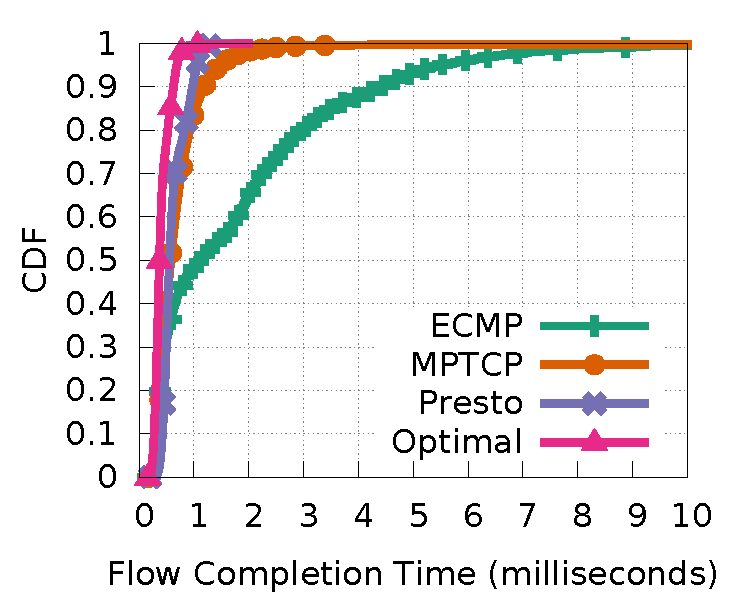
\includegraphics[width=0.45\textwidth]{presto/figures/macro/bijection/macro_compare_fct_bijection_mice.pdf}
        \caption{Macro evaluation - flow completiom time in Random Bijection workload}
        \label{macro_evaluation_fct_bijection}
\end{figure}

\begin{figure}[!t]
        \centering
  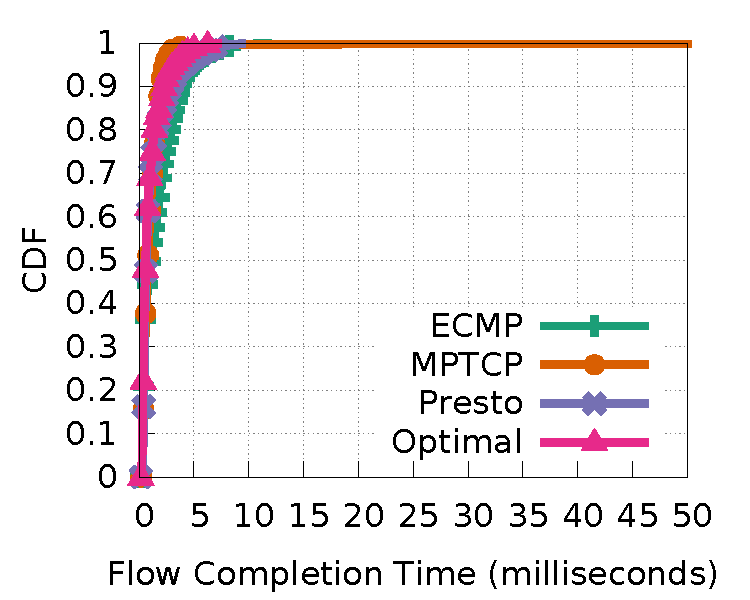
\includegraphics[width=0.45\textwidth]{presto/figures/macro/random/macro_compare_fct_random_mice.pdf}
        \caption{Macro evaluation - flow completiom time in Random workload}
        \label{macro_evaluation_fct_random}
\end{figure}


\begin{figure}[!t]
        \centering
  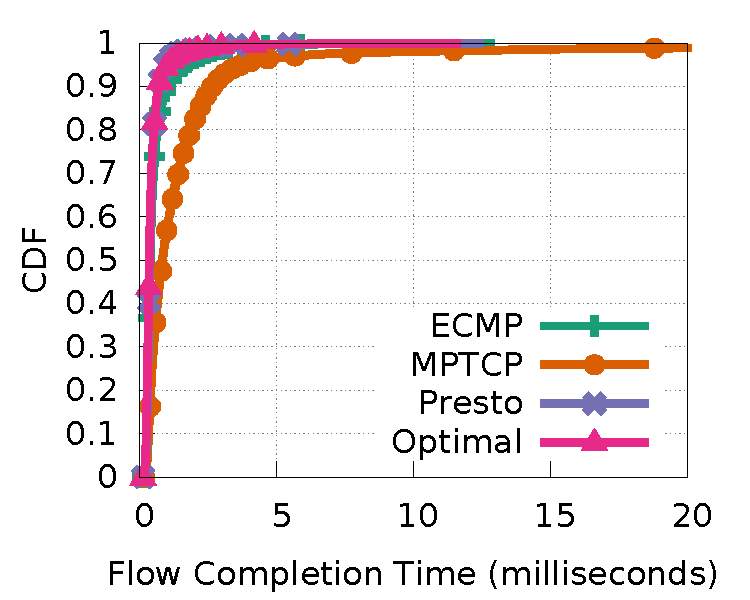
\includegraphics[width=0.45\textwidth]{presto/figures/macro/shuffle/macro_compare_fct_shuffle_mice.pdf}
        \caption{Macro evaluation - flow completiom time in Shuffle workload}
        \label{macro_evaluation_fct_shuffle}
\end{figure}

\fi

\iffalse
\begin{table}[!htb]
\begin{center}
\begin{tabular}{ |c|c|c|c|c| } 
 \hline
 Shuffle & ECMP & MPTCP & Presto & Optimal \\
 \hline 
 Median & 401 & 874 & 387 & 369  \\ 
 90\%   & 1037 & 2664 & 726 & 712 \\
 99\%   & 3373 & 21600  & 2447 & 2446 \\ 
 99.9\% & 12830 & 206ms & 12480 & 11714 \\
 %99.99\% & 204.1ms & - & 204.1ms & 203.6ms \\
 \hline

\end{tabular}
\caption{Macro evaluation - A close look of flow completiom time in Shuffle workload}
        \label{macro_evaluation_fct_shuffle_closelook}
\end{center}
\end{table}

\begin{table}[!htb]
\begin{center}
\begin{tabular}{ |c|c|c|c|c| }
 \hline
 Random & ECMP & MPTCP & Presto & Optimal \\
 \hline
 Median & 1008 & 780 & 648 & 595  \\
 90\%   & 3815 & 1918 & 2850 & 2297 \\
 99\%   & 7852 & 3380  & 6900 & 4936 \\
 99.9\% & 11784 & 202ms & 9372 & 7127 \\
% 99.99\% & 11677 & - & 16591 & 200ms \\
 \hline

\end{tabular}
\caption{Macro evaluation - A close look of flow completiom time in Random workload}
        \label{macro_evaluation_fct_random_closelook}
\end{center}
\end{table}

\fi

%%% trace-driven workload, MSR, scaling factor =10
\begin{table}[!tb]
\begin{center}
\begin{tabular}{ |c|c|c|c| }
 \hline
 Percentile & ECMP & Optimal &Presto \\
 \hline
 50\%   & $1.0$ & $-12\%$ & $-9\%$   \\
 90\%   & $1.0$ & $-34\%$ & $-32\%$  \\
 99\%   & $1.0$ & $-63\%$  & $-56\%$ \\
 99.9\% & $1.0$ & $-61\%$ & $-60\%$  \\
 \hline

\end{tabular}
\caption{Mice ($<$100KB) FCT in trace-driven workload~\cite{kandula2009nature}. Negative numbers imply shorter FCT.}
        \label{macro_evaluation_MSR_trace_driven}
\end{center}
\end{table}

\tightparagraph{Trace-driven Workload}
We evaluate Presto using a trace-driven workload based on traffic patterns measured in~\cite{kandula2009nature}. 
Each server establishes a long-lived TCP connection 
with every other server in the testbed. 
Then each server continuously samples flow sizes and inter-arrival times and each time sends to a random receiver
that is not in the same rack.
%Since 99\% of flows are less than 4MB in the distribution, 
We scale the flow size distribution by a factor of 10 to emulate a heavier workload. 
Mice flows are defined as flows that are less than 100 KB in size, and elephant flows are defined as flows
that are greater than 1 MB. The mice FCT, normalized to ECMP, 
is shown in Table~\ref{macro_evaluation_MSR_trace_driven}. 
Compared with ECMP, Presto has similar performance at the 50$^{th}$ percentile but reduces the 99$^{th}$ and 99.9$^{th}$ percentile FCT by 56\% and 60\%, respectively. 
Note MPTCP is omitted because its performance was quite unstable in workloads
featuring a large number of small flows.
The average elephant throughput (not shown) for Presto tracks Optimal (within 2\%), and improves upon ECMP by over 10\%.


\begin{table}[!htb]
\begin{center}
\begin{tabular}{ |c|c|c|c|c| }
 \hline
% Percentile & 50\% & 90\% & 99\% & 99.9\% \\
% \hline
% ECMP & 1.0 & 1.0 & 1.0 & 1.0  \\
% N-block   & 66\% & 17\% & 11\% & 9\% \\
% Presto    & 80\% & 21\% & 14\% & 10\% \\
% MPTCP     & 88\% & 27\% & 27\% & TIMEOUT \\

 Percentile & ECMP & Optimal & Presto & MPTCP \\
 \hline
 50\%       & 1.0 & $-34$\%     & $-20$\%   & $-12$\% \\
 90\%       & 1.0 & $-83$\%     & $-79$\%   & $-73$\% \\
 99\%       & 1.0 & $-89$\%     & $-86$\%   & $-73$\% \\
 99.9\%     & 1.0 & $-91$\%      & $-87$\%   & TIMEOUT \\

 \hline
\end{tabular}
\caption{FCT comparison (normalized to ECMP) with ECMP load balanced north-south traffic. Optimal means all the hosts are attached to a single  switch.}
	\label{macro_evaluation_north_south_traffic}
\end{center}
\end{table}


\tightparagraph{Impact of North-South Cross Traffic}
Presto load balances on "east-west" traffic in the datacenter, \ie{}, traffic
originating and ending at servers in the datacenter. 
In a real datacenter environment "north-south" traffic (\ie{}, traffic with an endpoint outside the datacenter)
must also be considered. 
%Ideally, north-south traffic should be load balanced by ECMP because of 
%reordering concerns at the end user. 
%However, east-west traffic typically dominates (75\% according to~\cite{east-west}). 
To study the impact of north-south traffic on Presto, we attach an additional server to 
each spine switch in our testbed to emulate remote users. 
The 16 servers establish a long-lived TCP connection with each remote user. 
Next, each server starts a flow to a random remote user every 1 millisecond. This emulates  
the behavior of using ECMP to load balance north-south traffic.
The flow sizes for north-south traffic are based on the distribution measurement in~\cite{he2013next}. 
The throughput to remote users is limited to 100Mbps to emulate the limitation of an Internet WAN. 
Along with the north-south flows, 
a stride workload is started to emulate the east-west traffic. 
The east-west mice FCT is shown in Table~\ref{macro_evaluation_north_south_traffic} (normalized to ECMP). 
ECMP, MPTCP, Presto, and Optimal's average throughput is 
5.7, 7.4, 8.2, and 8.9Gbps respectively. 
The experiment shows Presto can gracefully co-exist with north-south cross traffic
in the datacenter.


%%%failure handling experiments

\begin{figure}[!t]
        \centering
  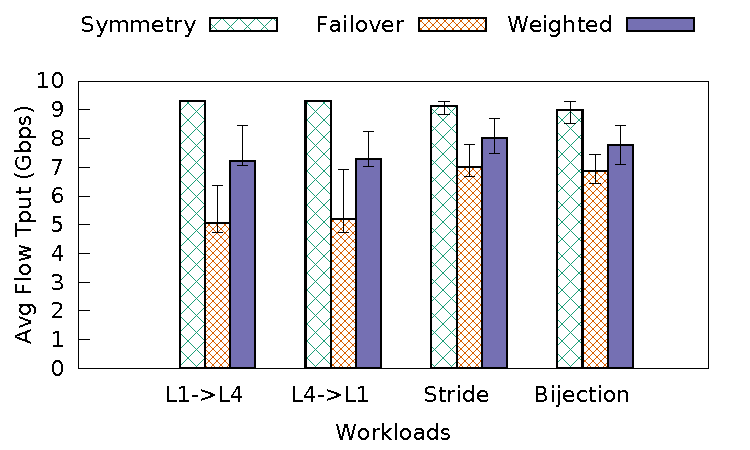
\includegraphics[width=0.7\textwidth]{presto/figures/failure_handling/failover_compare_tput_witherrbar.pdf}
        \caption{Presto's throughput in symmetry, failover and weighted multipathing stages for different workloads.}
        \label{failover_compare_tput}
\end{figure}

\begin{figure}[!t]
        \centering
  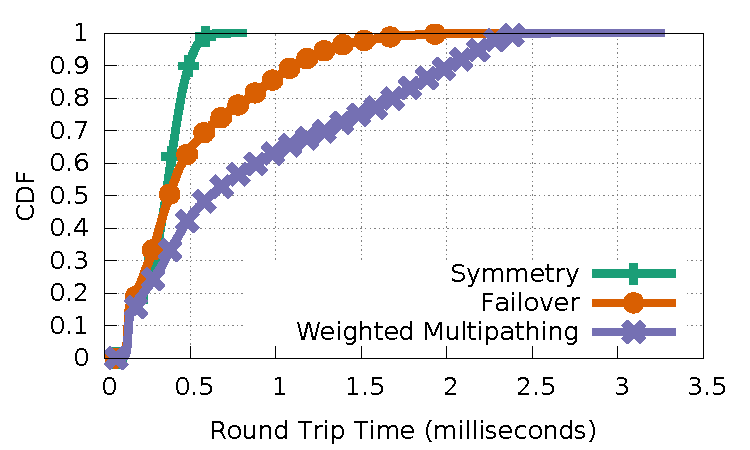
\includegraphics[width=0.7\textwidth]{presto/figures/failure_handling/failover_compare_sockperf_bijection_mice.pdf}
        \caption{Presto's RTT in symmetry, fast failover and weighted multipathing stages in  random bijection workload.}
        \label{failover_compare_sockperf_bijection}
\end{figure}

\tightparagraph{Impact of Link Failure}
Finally, we study the impact of link failure.
Figure~\ref{failover_compare_tput} compares the throughputs of
Presto when %under different stages of loss recovery when 
the link between spine switch S1 and leaf switch L1 goes down.
Three stages are defined: symmetry (the link is up), failover (hardware fast-failover moves traffic from S1 to S2), and weighted (the controller
learns of the failure and prunes the tree with the bad link).
Workload L1$\rightarrow$L4 is when each node connected to L1 sends to one node in L4 (L4$\rightarrow$L1 is the opposite).
Despite the asymmetry in the topology, Presto still achieves reasonable average throughput at 
each stage.
Figure~\ref{failover_compare_sockperf_bijection} shows the round trip time of
each stage in a random bijection workload. 
Due to the fact that the network is no longer non-blocking after the link failure,
failover and weighted multipathing stages have larger round trip time.



\iffalse
\begin{enumerate}
\item Clos-network, macro. ECMP, MPTCP, Presto and Optimal.
\begin{enumerate}
	\item Workloads: Take from Planck and Hedera. Can do MSR trace-based.
	\item Throughput, fairness, latency (maybe loss). Link utilization?
\end{enumerate}

\item Fat tree, macro. ECMP, MPTCP, Presto and Optimal.
\begin{enumerate}
        \item Workloads: Take from Planck and Hedera. Can do MSR trace-based.
        \item Throughput, fairness, latency (maybe loss). Link utilization?
\end{enumerate}


\item Vary flow sizes. Idea is that we can work on very small elephants.

\item Failure: backbone switch fails, aggregate switch fails, ToR switch fails, link fails, ...

\item CONGA uses incast, should we check?

\item Maybe this belongs in micro: ECMP vs shadowMAC for multipathing.

\end{enumerate}
\fi


{\bf Load Balancing in Datacenters} 
%Load balancing in datacenter networks has been the focus of several studies.
MPTCP~\cite{mptcp,dc-mptcp} is a transport protocol that uses subflows to 
transmit over multiple paths.
CONGA~\cite{conga} and Juniper VCF~\cite{juniper-vcf} both employ congestion-aware flowlet switching~\cite{flowlet} on
specialized switch chipsets to load balance the network.
RPS~\cite{packetspray} and DRB~\cite{drb} evaluate per-packet load balancing on symmetric 1 Gbps networks
at the switch and end-host, respectively.
The CPU load and feasibility of end-host-based per-packet load balancing for 10+ Gbps networks remains open.
%Per-packet load balancing can incur significant end-host overhead for DRB
%if not resorting to jumbo frames.
%Packet reordering problem is not well considered in both RPS and DRB.
%RPS and DRB may perform worse than ECMP in case of topology asymmetry.
Hedera~\cite{hedera}, MicroTE~\cite{microte} and Planck~\cite{planck} use centralized traffic engineering to
reroute traffic based on network conditions.
FlowBender~\cite{flowbender} reroutes flows when congestion is detected by end-hosts and 
Fastpass~\cite{fastpass} employs a centralized arbiter to schedule path selection for each packet.
As compared to these schemes, Presto is the only one that proactively load-balances at line rate for fast networks
in a near uniform fashion without requiring additional infrastructure or changes
to network hardware or transport layers. Furthermore, to the best of our knowledge, Presto is
the first work to explore the interactions of fine-grained load balancing with built-in
segment offload capabilities used in fast networks.
%\textcolor{blue}{~\cite{eden} also advocates to implement network functions such as load balancing 
%at datacenter end hosts.}

{\bf Reducing Tail Latency}
%Detail~\cite{detail} summarizes the causes of long tails of flow completion time---
%1)packet loss and retransmissions,
%2)absence of flow prioritization and 3)uneven load balancing.
%Reducing tail latencies of small mice flows has also been actively studied.
DeTail~\cite{detail} is a cross-layer network stack designed to reduce the tail of flow completion times.
%link layer uses port buffer occupancy to construct lossless fabric,
%network layer performs per-packet adaptive load balancing based on port buffer occupancy,
%transport layer relies upon congestion notifications
%derived from port buffer occupancies,
%finally Detail lets application layer specify flow priorities to
%avoid head-of-line blocking of elephant flows for mice time-sensitive flows.
%Detail modified many layers (including the switch) and is hard to deploy using
%current hardware and network stack.
DCTCP~\cite{dctcp} is a transport protocol that uses the portion of marked packets 
by ECN to adaptively adjust sender's TCP's congestion window to reduce switch buffer occupancy.
%Thus, DCTCP can reduce switch buffer occupancy and reduce flow completion time.
HULL~\cite{hull} uses Phantom Queues and congestion notifications to cap link utilization and prevent congestion.
%HULL uses packet pacing to combat with traffic burstiness in order to leave "bandwidth headroom".
In contrast, Presto is a load balancing system that naturally improves 
the tail latencies of mice flows by uniformly spreading traffic in 
fine-grained units.
%We share the overall goal of reducing mice tail latencies, but instead explore how
%fine-grained load balancing can provide a solution.
QJUMP~\cite{qjump} utilizes priority levels to 
allow latency-sensitive flows to "jump-the-queue" over low priority flows.
PIAS~\cite{bai2015information} uses priority queues to mimic the Shortest Job First principle to reduce FCTs.
%solve the network interference problem caused by elephant and mice flows 
%for datacenter networks. High priority packets are rate-limited 
%at the end-host and can "jump-the-queue" over packets with 
%lower priorities. PIAS~\cite{pias} mimics the Shortest Job First (SJF) 
%principle to reduce flow completion times. It gradually decreases 
%the priority level assigned to a flow based on its flow size.
%Presto is complementary and could be applied on each priority level.
%DIBS~\cite{dibs} detours packets of a congested switch port to a randomly 
%picking neighboring switch to reduce packet drops.
Last, a blog post by Casado and Pettit~\cite{vmware} summarized
four potential ways to deal with elephants and mice, with one advocating
to turn elephants into mice at the edge. 
We share the same motivation and high-level
idea and design
a complete system that addresses many practical challenges of using
such an approach.


{\bf Handling Packet Reordering}
%Many schemes have tried to mitigate the impact of reordering.
TCP performs poorly in the face of reordering, and thus several studies
design a more robust alternative~\cite{rr-tcp,blanton2002making,tcp-pr}.
Presto takes the position that reordering should be handled below TCP in the existing 
receive offload logic.
In the lower portion of the networking stack, SRPIC~\cite{wu2009sorting} sorts reordered packets 
in the driver after each interrupt coalescing event. While this approach can help
mitigate the impact of reordering, it does not sort packets across interrupts, have a 
direct impact on segment sizes, or distinguish between loss and reordering. 
%SRPIC is 
%complementary to our approach because their actions are taken in the driver, before packets
%are pushed to GRO.
%RR-TCP~\cite{rr-tcp} proposed to extend TCP sender to detect and recover from false fast retransmits using DSACK information. 
%As we show, fixing TCP itself cannot solve all the problems incurred by packet reordering.
%\eric{i have some LRO references in the patent slides that we need to make sure are cited somewhere} 
%Instead, Presto's chunking scheme leverages the fact that all the packets going through the same path are in order and has two nice properties:
%1)Presto uses chunkid to make the task of distinguishing packet loss from temporary packet reordering much simpler. 
%2)Presto only needs to make sure the chunks are in order instead of packets, thus reducing per-packet processing overhead.

{\bf Congestion control for DCNs}
%\crs{Rather than proposing a new congestion control algorithm, our work investigates if congestion control can be moved to the vSwitch.
%Thus, many of the following schemes are complimentary.}
DCTCP~\cite{dctcp} is a seminal TCP variant for datacenter networks.
Judd~\cite{judd2015nsdi} proposed simple yet practical fixes to enable DCTCP in production networks.
TCP-Bolt~\cite{stephens2014practical} is a variant of DCTCP for PFC-enabled lossless Ethernet.
%DCQCN~\cite{zhu2015congestion} is a rate-based congestion control scheme implemented in NICs
%for QCN-based~\cite{qcn} RDMA deployments.
DCQCN~\cite{zhu2015congestion} is a rate-based congestion control scheme (built on DCTCP and QCN) to
support RDMA deployments in PFC-enabled lossless networks.
TIMELY~\cite{mittal2015timely} and DX~\cite{lee2015accurate}
use accurate network latency as the signal to perform congestion control.
TCP ex Machina~\cite{winstein2013tcp} uses computer-generated congestion control rules.
PERC~\cite{jose2015high} proposes proactive congestion control to improve convergence.
ICTCP's~\cite{wu2010ictcp} receiver monitors incoming TCP flows and
modifies~\rwnd{} to mitigate the impact of incast, but this cannot
provide generalized congestion control like~\acdc{}.
Finally, efforts~\cite{dell-toe,chelsio-toe} to
implement TCP Offload Engine (TOE) in specialized NICs are not widely deployed for reasons noted in~\cite{mogul2003tcp,linux-toe}.
vCC~\cite{vcc} is a concurrently designed system that shares~\acdc{}'s goals and some of its design details.
The paper is complementary in that some items not addressed in~\acdc{} are presented, such as a more detailed
analysis of the ECN-coexistence problem, an exploration of the design space, and a theoretical proof of
virtualized congestion control's correctness.~\acdc{} provides an in-depth design and thorough evaluation of
a DCTCP-based virtualized congestion control algorithm on a 10 Gbps testbed.


{\bf Bandwidth allocation} Many bandwidth allocation schemes have been proposed.
Gatekeeper~\cite{rodrigues2011gatekeeper} and EyeQ~\cite{jeyakumar2013eyeq} abstract the network as a single
switch and provide bandwidth guarantees by managing each server's access link.
Oktopus~\cite{Ballani2011oktopus} provides fixed performance guarantees within virtual clusters.
SecondNet~\cite{Guo2010Secondnet} enables virtual datacenters with static bandwidth guarantees.
Proteus~\cite{Xie2012Proteus} allocates bandwidth for applications with dynamic demands.
Seawall~\cite{shieh2011sharing} provides bandwidth proportional to a defined weight by
forcing traffic through congestion-based edge-to-edge tunnels.
NetShare~\cite{Lam2012NetShare} utilizes hierarchical weighted max-min fair sharing to tune relative bandwidth allocation for services.
FairCloud~\cite{Popa2012Faircloud} identifies trade-offs in minimum
guarantees, proportionality and high utilization, and designs schemes over this space.
Silo~\cite{jang2015silo} provides guaranteed bandwidth, delay and burst allowances through a novel VM placement and admission
algorithm, coupled with a fine-grained packet pacer. 
~\acdc{} is largely complimentary to these schemes because it is a transport-level solution.

{\bf Rate limiters}
SENIC~\cite{niranjan2013fastrak}
identifies the limitations of NIC hardware rate limiters (\ie{}, not scalable) and
software rate limiters (\ie{}, high CPU overhead) and uses the CPU to enqueue packets
in host memory and the NIC. Silo's pacer injects void packets into
an original packet sequence to achieve pacing. FasTrack~\cite{niranjan2013fastrak} offloads
functionality from the server into the switch for certain flows.
%~\acdc{} prevents
%TCP flows from sending in the first place and can be used in conjunction with these
%schemes.


%\section{Discussion}
\label{discuss}

\tightparagraph{UDP traffic} How to handle. 
Mention VxLAN traffic too.
\keqiang{and IPsec}

\tightparagraph{No vSwitch} 
\keqiang{title should be hypervisor-bypass?}
Use middleboxes (for DB server).
Use NIC (for SR-IOV).
Hypervisor bypass (e.g., SR-IOV), where TCP traffic is sent to the NIC directly without 
going through hypervisor. First, as noted by~\cite{shieh2011sharing}, ``loss of the security and 
manageability features provided by the software virtual switch has limited 
the deployment of direct I/O NICs in public clouds''. Second, based on techniques like Intel 
DPDK~\cite{intel-dpdk} and ``smart NICs''~\cite{cavium-nic,netronome-nic}, we believe that low latency 
congestion control enforcement schemes like \acdc{} can also be 
employed for hypervisor bypass use cases.
We need to worry about legacy systems and non-VM systems. For instance, a database or storage device that may not have OVS installed on it.
We need to talk about either a middlebox or that this percentage of traffic is low? Or implement in NIC (especially one with OVS offload?).

\tightparagraph{North-South traffic.}
Transport enforcement should be only be done for east west traffic, so if the tenant tuned their stack's
congestion control algorithm for wide-area networks, their north sourth traffic is not affected and their 
congestion control scheme can still achieve good performance.

\keqiang{todos: some figures do not read well on printed paper}
\keqiang{todos: sometimes, when we refer a section, we say ``Section X'', sometimes, we use the 
dollar sign, we should unify them}

%
%Byzantine VM.
%
%Other names: ACDCTCP, LiquidSwitch, LiquidEdge
%
%In CPU overhead measurement, we need to 
%mention ovs add 1 widecard rule. That means we isolated the overhead of 
%OVS itself when it has many flows in its flow table (probably it does not matter
%at the end of the day, because we measured the CPU usage of the whole system).
%
%People may say window-based congestion control is burty. TIMELY operates 
%on TCP segments in order to reduce CPU overhead. Therefore, TIMELY is also
%busty. In TIMELY, they mentioned they can leverage a hybrid scheme, that is
%using software to control large segments and use hardware rate limiter to
%reduce burstyness.
%
%Create loss and check how DCTCP and our scheme treates packet losses (revisit it after we finish incast 
%and macrobenchmarks).
%
%One more microbenchmark on the Dumbbell topology: different servers have different transport, so the
%throughput fairness among different transports (e.g., start cubic, start New Reno, start dctcp).
%
%A point that is missing in DCTCP and NSDI paper is that they did not mention how the switch should be
%configured to handle non-TCP traffic. Note non-TCP traffic such as DNS (UDP 53) and ARP, ICMP etc
%are also important. We found that if we did not specify how the switch handle the non-TCP traffic,
%then this kind of non-TCP traffic can be easily dropped by the switch. We found ARP traffic is dropped
%by the switch such that DCTCP flows stall. Hence, we think it is better to put non-TCP traffic
%into a different queue when we apply WRED/ECN on the switches.
%
%This work offers low latency for ``hetergeneous networks" where different entities can 
%run different kinds of
%transport congestion control schemes. A few examples of such hetergeneous networks: public 
%datacenters where tenants can set up their own VMs (e.g., AWS), or tenants can rent their bare metal
%machines (e.g., SoftLayer), or certain groups (even within a single organization) 
%have to use traditional transports due to compatibility of legacy applications (NSDI's Judd said this), or
%incremental deployment is undergoing. 
%To ensure a pure low latency datacenter network, a universal transport enforcement scheme is required. 
%Two challenges to implement such a transport enforcement scheme are scalability and low overhead. 
%The transport enformancement scheme proposed here meet the two metrics (as shown in our experiments) while
%providing nice network performance (throughput, latency and packet drop rate). This scheme is 
%compatible with any kind of TCP stack. Finally, the scheme we propose solves the co-existence issue of 
%ECT (ECN Capable Transport) and non-ECT, which is a critical deployment hurdle for DCTCP-like transports.
%
%Macrobenchmark plan: 18 hosts, 6 switches, ECMP configured. The network oversubscription ratio is 2:1.
%Run all-to-all traffic for a long time (e.g., 1 hours). Show total throughput and TCP RTT and packet drop 
%rate.
%
%QoS can be implemented too?
%
%
%
%When we try to launch an instance in EC2: ``An AMI is a template that contains the software 
%configuration (operating system, application server, and applications) required to launch your instance. 
%You can select an AMI provided by AWS, our user community, or the AWS Marketplace; 
%or you can select one of your own AMIs''. Default is CUBIC for most Linux images, Window Servers can
%have NewReno, Compound TCP (CTCP)~\cite{tan2006compound} and DCTCP. 
%Users can tweak congestion control algorithms to optimize network performance for their target scenarios. 
%
%Section talking about how to implement other CC schemes: TIMELY, PERC, Vegas, etc.
%
%EJR: VXLAN, UDP, TCP stack statistics for Cloud?
%
%ECT and non-ECT: througput unfairness, long RTT, connection establishment..
%
%
%EyeQ, Seawall, NetShare, Silo, SecondNet, Oktopus etc. Our work did not provide bandwidth allocation property. 
%This work focused on reducing in-network queuing latency caused by VM TCP stacks. 
%We show how this goal can be done using a simple and elegant solution.
%Yes, if an VM opens more connections than another, that VM gains more bandwidth. 
%But, there are proposals which try to provide proper bandwidth allocation when multiple end-points compete 
%at the sender side or receiver side. Those works and this work are complementary. 
%To the best of our knowledge, today's cloud providers have not provide strong bandwidth guarantees 
%(for example, AWS only roughly classify VMs instances' network performance into 
%``low to moderate", ``moderate", ``high" and ``10 Gigabit"categories).
%
%talk about containers?

\section{Summary}
\label{sec:conclusion}
In this chapter, we present Presto: a near uniform sub-flow distributed load balancing scheme
that can near optimally load balance the network at fast networking speeds.
Our scheme makes a few changes to the hypervisor soft-edge (vSwitch and GRO)
and does not require any modifications to the transport layer or network hardware, making
the bar for deployment lower. 
%Working at fast networking speeds poses many challenges,
Presto is explicitly designed to load balance the network at fine granularities
and deal with reordering without imposing much overhead on hosts. Presto is flexible and can also
deal with failures and asymmetry. Finally, we show the performance of Presto can closely track
that of an optimal non-blocking switch, meaning elephant throughputs remain high while the tail
latencies of mice flow completion times do not grow due to congestion.


\section*{Acknowledgement}

We would like to thank Jon Crowcroft (our shepherd) and
the anonymous reviewers for their valuable feedback. This
work is supported in part by IBM Corporation, National
Science Foundation (grants CNS-1302041, CNS-1330308
and CNS-1345249) and the Wisconsin Institute on Software-Defined Datacenters of Madison.
{
%\scriptsize
\small
\setlength{\bibsep}{0.5pt}
\raggedright
\balance
\bibliographystyle{abbrv}
\bibliography{refer}
}

\end{document}
